\documentclass[11pt,a4paper]{article}

% ----------------------------------------------------------------------
%  Hydrophone measurement of MI and acoustic intensities -- a protocol
% ----------------------------------------------------------------------
% inputenc is unnecessary on modern LaTeX (UTF-8 is the default) and breaks
% non-ASCII glyphs such as \micro under XeTeX/LuaTeX -- do not re-add it.
\usepackage[T1]{fontenc}
\usepackage{lmodern}
\usepackage[margin=2.4cm]{geometry}
\usepackage{graphicx}
\usepackage{booktabs}
\usepackage{amsmath}
\usepackage{siunitx}
\usepackage{xcolor}
\usepackage{caption}
\usepackage{subcaption}
\usepackage{enumitem}
\usepackage{microtype}
\usepackage{array}
\usepackage{longtable}
\usepackage{mdframed}
\usepackage{tikz}
\usetikzlibrary{arrows.meta,positioning}
\usepackage[hidelinks,colorlinks=true,linkcolor=blue!55!black,citecolor=blue!55!black,urlcolor=blue!55!black]{hyperref}

\graphicspath{{figures/}}
\captionsetup{font=small,labelfont=bf}
\setlist{itemsep=2pt,topsep=3pt}

\newcommand{\good}[1]{\textcolor{green!45!black}{\textbf{#1}}}
\newcommand{\caveat}[1]{\textcolor{orange!75!black}{\textbf{#1}}}
\newcommand{\todoitem}[1]{\textcolor{red}{\textbf{[TODO: #1]}}}
\sisetup{detect-weight=true,detect-family=true}
\DeclareSIUnit{\sample}{S}
% siunitx 3.0.x declares the micro prefix as a literal U+00B5. Under T1 that
% slot is t-with-cedilla, so every \micro came out as a stray letter. The math
% mu is always available and renders correctly on every engine.
\DeclareSIPrefix{\micro}{\ensuremath{\mu}}{-6}

% a boxed "common mistake" callout
\newmdenv[linecolor=orange!70!black,linewidth=0.8pt,backgroundcolor=orange!4,
          leftmargin=0pt,rightmargin=0pt,innertopmargin=5pt,innerbottommargin=5pt,
          skipabove=7pt,skipbelow=7pt]{mistake}
\newcommand{\mistaketitle}[1]{\textcolor{orange!75!black}{\textbf{Common mistake --- #1}}\\[2pt]}

% flowchart styles (used by flowchart.tex).
% NB: do not call these 'step'/'watch' -- /tikz/step is a built-in key (grid step)
% and TikZ's definition wins, which silently strips the box and the line breaks.
\tikzset{
  pstep/.style = {rounded corners=3pt, draw=blue!55!black, fill=blue!5, line width=0.7pt,
                  text width=7.0cm, align=left, inner sep=5pt, font=\small},
  pwatch/.style= {rounded corners=2pt, draw=orange!75!black, fill=orange!6, dashed,
                  line width=0.6pt, text width=5.4cm, align=left, inner sep=4pt,
                  font=\footnotesize},
  flow/.style  = {-{Latex[length=2.4mm]}, draw=blue!55!black, line width=0.8pt},
  hint/.style  = {densely dotted, draw=orange!75!black, line width=0.5pt},
}

\title{\vspace{-1.5em}\textbf{Measuring the Mechanical Index and Acoustic Intensities\\
of a Custom Verasonics Sequence}\\[0.4em]
\large Hydrophone measurement protocol}
\author{TU Eindhoven --- Shear-wave elastography}
\date{September 2026}

\begin{document}
\maketitle

\begin{abstract}
\noindent
Any custom transmit sequence used on a subject must be shown to stay inside the accepted
acoustic-output limits. The Verasonics software reports these for a handful of its own example
scripts, but not for sequences we write ourselves, and not for the long ARF pushes used in
shear-wave elastography --- so they have to be measured. This document is a protocol for doing that
with a calibrated hydrophone: what the setup is (\S\ref{sec:equipment}), how to capture a voltage
correctly (\S\ref{sec:voltage}), how to convert it to MI, $I_\mathrm{sppa.3}$ and
$I_\mathrm{spta.3}$ (\S\ref{sec:conversion}), and the step-by-step measurement itself
(\S\ref{sec:protocol}); Figure~\ref{fig:flow} is the whole thing on one page.
\S\ref{sec:approach} sets out both the \emph{ideal} measurement --- a full
3-D raster of the field --- and the reduced one-dimensional measurement that is actually described
here, and what it costs. \S\ref{sec:checklist} collects the mistakes that are easy to make and
expensive to discover late. \S\ref{sec:results} gives worked results from our own L11-5 and S5-1
measurements as examples of what the output looks like, and Appendix~\ref{app:owis} covers the
motion stage the hydrophone is mounted on.
\end{abstract}

\tableofcontents

% ----------------------------------------------------------------------
%  Symbols and abbreviations.
%  Unnumbered (\section*) on purpose: numbering it would shift every section
%  number in the document, and the code and READMEs cite those numbers.
%  Included from main.tex, immediately after the table of contents.
% ----------------------------------------------------------------------
\section*{Symbols and abbreviations}
\addcontentsline{toc}{section}{Symbols and abbreviations}

\noindent
The equations in \S\ref{sec:intro} and \S\ref{sec:conversion} use these throughout. A subscript
$.3$ on any acoustic quantity means it has been \textbf{derated} by
\SI{0.3}{\decibel\per\centi\metre\per\mega\hertz} to emulate the attenuation of intervening tissue;
without it the quantity is the one measured in water.

\newcommand{\nomrow}[2]{#1 & #2 \\}

\begingroup
\small
\setlength{\tabcolsep}{5pt}
\renewcommand{\arraystretch}{1.18}

\begin{longtable}{@{}p{0.20\textwidth}p{0.74\textwidth}@{}}
\endhead
\multicolumn{2}{@{}l}{\textbf{The regulated quantities}}\\
\midrule
\nomrow{MI}{Mechanical index, $p_\mathrm{r.3}/\sqrt{f_\mathrm{awf}}$. A \emph{cavitation} index: the
  potential for mechanical damage. Dimensionless.}
\nomrow{$I_\mathrm{sppa.3}$}{Spatial-peak \emph{pulse-average} intensity, $\mathrm{PII}_{.3}/\mathrm{PD}$
  [\si{\watt\per\square\centi\metre}]. A \emph{thermal} quantity: how hard one pulse heats.}
\nomrow{$I_\mathrm{spta.3}$}{Spatial-peak \emph{time-average} intensity,
  $\mathrm{PII}_{.3}\cdot\mathrm{PRF}$ [\si{\milli\watt\per\square\centi\metre}]. The long-time
  average, so it depends on how often you transmit.}
\nomrow{TI}{Thermal index. Not measured here; mentioned because $I_\mathrm{spta}$ does not capture
  the temperature rise \emph{within} a burst (\S\ref{sec:scaling}).}
\addlinespace[4pt]

\multicolumn{2}{@{}l}{\textbf{What goes into them}}\\
\midrule
\nomrow{$p_r$}{Peak rarefactional pressure [\si{\mega\pascal}]: the most negative excursion of the
  pressure waveform. \emph{Not} $V_\mathrm{pp}/2$ --- the waveform is asymmetric.}
\nomrow{$p_+$}{Peak compressional pressure: the most positive excursion. Reported for context; no
  index uses it.}
\nomrow{$f_\mathrm{awf}$}{Acoustic working frequency [\si{\mega\hertz}]: the centre of the
  \SI{-6}{\decibel} band of the fundamental (\S\ref{sec:fawf}). Measure it, do not assume the
  programmed transmit frequency.}
\nomrow{PII}{Pulse intensity integral [\si{\joule\per\square\metre}], $\int p^2/(\rho c)\,dt$ over
  the pulse.}
\nomrow{PD}{Pulse duration [\si{\second}], $1.25\,(t_{90}-t_{10})$.}
\nomrow{$t_{10}$, $t_{90}$}{The instants at which the cumulative intensity integral reaches
  \SI{10}{\percent} and \SI{90}{\percent} of its final value.}
\nomrow{PRF}{Pulse repetition frequency [\si{\hertz}]. A property of the \emph{sequence}, not of a
  capture. For a burst protocol use the \emph{effective} rate.}
\nomrow{$\rho$, $c$}{Density and speed of sound of the medium; \SI{1000}{\kilo\gram\per\cubic\metre}
  and \SI{1500}{\metre\per\second} throughout.}
\nomrow{$z$}{Depth [\si{\centi\metre}]: distance from the transducer face to the measurement point,
  $\lVert\mathtt{Pos}-\mathtt{Home}\rVert$ (\S\ref{sec:home}). Sets the derating.}
\addlinespace[4pt]

\multicolumn{2}{@{}l}{\textbf{The hydrophone chain} (\S\ref{sec:calibration})}\\
\midrule
\nomrow{$M_c(f)$}{\textbf{Open-circuit} end-of-cable hydrophone sensitivity [\si{\volt\per\pascal}]
  --- what the Onda certificate gives. Not what the scope sees.}
\nomrow{$M_L(f)$}{\textbf{Loaded} system sensitivity [\si{\volt\per\mega\pascal}] --- $M_c$ after the
  capacitive divider and any gain. This is what converts volts to pressure.}
\nomrow{$G(f)$}{Gain of the AH-2010 pre-amplifier ($\approx\SI{20}{\decibel}$), referenced to a
  \SI{50}{\ohm} load.}
\nomrow{$C_H$}{Hydrophone element capacitance, $\approx\SI{12.7}{\pico\farad}$.}
\nomrow{$C_A$}{Pre-amplifier input capacitance, \SI{6.1}{\pico\farad}. Loads the hydrophone on
  chain~A.}
\nomrow{$C_\mathrm{load}$}{Cable $+$ scope capacitance, $\approx\SI{123}{\pico\farad}$. Loads the
  hydrophone on chain~B, where it dominates. Not a datasheet value --- measure it
  (\S\ref{sec:cloadcal}).}
\nomrow{$R_L$}{Oscilloscope input impedance, \SI{50}{\ohm} or \SI{1}{\mega\ohm}
  (\S\ref{sec:impedance}).}
\nomrow{$R_\mathrm{out}$, $R_\mathrm{ref}$}{Pre-amplifier output impedance and the load its
  calibration is referenced to; both \SI{50}{\ohm}.}
\nomrow{$V_A$, $V_B$}{The same acoustic point read on chain~A and chain~B.}
\nomrow{$V_\mathrm{pp}$}{Peak-to-peak voltage of a capture.}
\nomrow{Chain A}{Hydrophone $\rightarrow$ pre-amplifier $\rightarrow$ scope. Sensitive; clips at
  $\approx\SI{2.2}{\volt}$ (\S\ref{sec:clipping}).}
\nomrow{Chain B}{Hydrophone $\rightarrow$ scope, pre-amplifier removed. $73\times$ less sensitive;
  no ceiling (\S\ref{sec:nopreamp}).}
\addlinespace[4pt]

\multicolumn{2}{@{}l}{\textbf{Beam geometry} (\S\ref{sec:stepsize})}\\
\midrule
\nomrow{$\lambda$}{Acoustic wavelength at $f_\mathrm{awf}$.}
\nomrow{$F_\#$}{f-number of the transmit beam, focal depth divided by active aperture.}
\nomrow{FWHM}{Full width at half maximum of the beam, $\approx1.21\,\lambda F_\#$ in the focal
  plane. The transverse search step is expressed as a fraction of it.}
\nomrow{$\Delta$}{Transverse scan step.}
\nomrow{\texttt{Home}, \texttt{Pos}}{Stage coordinates of the transducer face centre and of the
  hydrophone tip, written into every capture note.}
\addlinespace[4pt]

\multicolumn{2}{@{}l}{\textbf{Abbreviations}}\\
\midrule
\nomrow{ARF}{Acoustic radiation force --- the long, high-amplitude push that drives a shear wave.}
\nomrow{FDA}{US Food and Drug Administration; the source of the output limits used here.}
\nomrow{IEC}{International Electrotechnical Commission; defines $f_\mathrm{awf}$ and the derating.}
\nomrow{\texttt{.hws}}{Hierarchical Waveform Storage, the NI capture format. HDF5 underneath.}
\nomrow{SFP}{Soft Front Panel, the NI application that drives the digitizer and writes
  \texttt{.hws}.}
\nomrow{ADC}{Analogue-to-digital converter. The PCI-5112 is \textbf{8-bit}, which is why the
  vertical range must be set tightly.}
\nomrow{RIS}{Random interleaved sampling: equivalent-time sampling, valid only for repetitive
  signals and \textbf{never} for a single-shot push (\S\ref{sec:scopesettings}).}
\bottomrule
\end{longtable}
\endgroup


% ======================================================================
\section{What has to be measured}\label{sec:intro}
% ======================================================================
Three quantities are regulated. All are defined at the \emph{spatial peak} of the field, and all are
\emph{derated} by \SI{0.3}{\decibel\per\centi\metre\per\mega\hertz} to emulate the attenuation of
intervening tissue (the subscript $.3$):

\begin{align}
  \mathrm{MI}          &= \frac{p_\mathrm{r.3}}{\sqrt{f_\mathrm{awf}}}
    & &\text{peak rarefactional pressure [\si{\mega\pascal}] over $\sqrt{f}$ [\si{\mega\hertz}]},
    \label{eq:mi}\\
  I_\mathrm{sppa.3}    &= \frac{\mathrm{PII}_{.3}}{\mathrm{PD}}
    & &\text{pulse-average intensity}, \label{eq:isppa}\\
  I_\mathrm{spta.3}    &= \mathrm{PII}_{.3}\cdot \mathrm{PRF}
    & &\text{time-average intensity}. \label{eq:ispta}
\end{align}

MI is a \textbf{cavitation} (mechanical) index; the two intensities are \textbf{thermal}. All symbols
are defined in \S\ref{sec:conversion}.

\subsection{The limits}\label{sec:limits}
The FDA guidance\footnote{\emph{Marketing Clearance of Diagnostic Ultrasound Systems and Transducers},
FDA, 2023; a copy is in \texttt{docs/datasheets/}.} sets application-specific limits
(Table~\ref{tab:fdalimits}). Pick the row for the intended use and compare against it.

\begin{table}[h]
\centering
\small
\caption{FDA acoustic output limits by application. Note the \textbf{or} in the last two columns:
formally a device needs $I_\mathrm{spta.3}$ below its limit \emph{and} either MI or
$I_\mathrm{sppa.3}$ below theirs. Satisfying \emph{both} is the conservative choice and is what is
assumed throughout this document.}
\label{tab:fdalimits}
\begin{tabular}{lccc}
\toprule
Use & $I_\mathrm{spta.3}$ (\si{\milli\watt\per\square\centi\metre})
    & $I_\mathrm{sppa.3}$ (\si{\watt\per\square\centi\metre}) & \textbf{or} MI \\
\midrule
Peripheral vessel        & 720 & 190 & 1.9 \\
Cardiac                  & 430 & 190 & 1.9 \\
Fetal imaging \& other   &  94 & 190 & 1.9 \\
Ophthalmic               &  17 &  28 & 0.23 \\
\bottomrule
\end{tabular}
\end{table}

\noindent
\textbf{Cardiac} covers transthoracic adult and paediatric use; \textbf{peripheral vessel} includes
the vessels of the neck; \textbf{fetal imaging \& other} is the catch-all (abdominal, small organ,
musculoskeletal, neonatal and adult cephalic). Transcranial use above
\SI{94}{\milli\watt\per\square\centi\metre} additionally requires an estimate of the maximum
temperature rise from a model that accounts for skull heating.

One caveat on what these numbers are for: the FDA compliance policy explicitly \textbf{excludes
shear-wave elastography}, and assumes 1--100 cycles per pulse --- a 1500--1900-cycle ARF push is an
order of magnitude outside that. For an ARF sequence, Table~\ref{tab:fdalimits} is therefore a
\textbf{benchmark rather than a compliance route}: these are the right quantities to measure and the
right targets to stay under, but the approval route is the medical-ethics committee.

\begin{mistake}
\mistaketitle{quoting ``the'' limit without saying which application}
$I_\mathrm{spta.3}$ ranges over $40\times$ across the rows of Table~\ref{tab:fdalimits} ---
\SI{720}{\milli\watt\per\square\centi\metre} for peripheral vessel against
\SI{17}{\milli\watt\per\square\centi\metre} for ophthalmic. State the application alongside every number you report, and when it is
not settled which applies, report against the stricter one.
\end{mistake}

\subsection{What changes what}
This table is worth internalising before planning a measurement, because it determines what must be
measured and what can be scaled:

\begin{center}
\begin{tabular}{lccc}
\toprule
Change & MI & $I_\mathrm{sppa.3}$ & $I_\mathrm{spta.3}$ \\
\midrule
Transmit voltage $V$            & $\propto V$ & $\propto V^2$ & $\propto V^2$ \\
Pulse length (\# cycles)        & unchanged   & unchanged     & $\propto$ cycles \\
PRF / duty cycle                & unchanged   & unchanged     & $\propto$ PRF \\
Aperture (\# elements), focused & $\approx\propto N$ & $\approx\propto N^2$ & $\approx\propto N^2$ \\
Beam type, focal depth          & \multicolumn{3}{c}{changes the field shape --- must be re-measured} \\
\bottomrule
\end{tabular}
\end{center}

\noindent
The pulse-length row is why a long ARF push is ``free'' on MI, and why long pushes tend to be limited
by $I_\mathrm{sppa.3}$ rather than by MI. The first three rows are what allow a single measurement at
the field maximum to be extrapolated instead of re-measuring the whole field for every variant.

% ======================================================================
\section{Two ways to do this}\label{sec:approach}
% ======================================================================

\subsection{The ideal measurement: a full 3-D raster}\label{sec:ideal}
What one really wants is the acoustic field \emph{sampled on a 3-D grid}, with several waveforms
saved at every grid point. Every quantity then follows without assumption: the spatial peak is simply
the maximum over the volume, the beam width and cross-sectional area come out for free (needed for
the spatial-averaging correction and for the thermal indices), the repeatability at each point is
measured rather than estimated, and no search algorithm has to converge on anything.

The hardware for this already exists in the setup. \textbf{OWIsoft supports a meander function} that
drives the stage through a predefined grid (Appendix~\ref{app:owis}), so the motion side is solved. \good{The only real
obstacle is synchronisation:} the Verasonics, the stage and the digitizer must be coordinated so
that, at every grid point, the stage settles, the sequence transmits, and the scope captures and
stores several records under a filename carrying the coordinates. Sketching what that needs:

\begin{itemize}
  \item a \textbf{position-reached signal} from the stage (a TTL output, or a polled status flag over
    the OWIsoft interface) to gate acquisition, so that no capture is taken while the stage is
    moving or still ringing down;
  \item \textbf{programmatic scope control} instead of the Soft Front Panel --- arm, capture $N$
    records, write to a file named by grid index --- driven from the same script that steps the
    meander;
  \item a \textbf{dwell time} per point long enough for the stage to settle and for $N$ transmit
    events to occur, which sets the total scan duration: a $20\times20\times20$ grid at
    \SI{2}{\second} per point is over four hours, so the grid extent and step have to be chosen with
    that in mind;
  \item a \textbf{coordinate log} written by the same script, so that positions are never inferred
    afterwards.
\end{itemize}

\caveat{This has not been built.} It is a significant piece of integration work and there was no time
for it. It is the right thing to build if these measurements are going to be repeated often, and
this section exists so that whoever picks it up knows the pieces are all present.

\subsection{The practical measurement: an axial line with a local transverse search}
In the absence of that synchronisation, the measurement described in this document reduces the 3-D
raster to a line: step along the beam axis, and at each axial station move laterally and in elevation
by hand (or by short stage moves) to find the local maximum, saving only that peak waveform. This is
a poor-man's version of the ideal scan and it should be understood as such.

\begin{center}
\begin{tabular}{p{0.30\textwidth}p{0.30\textwidth}p{0.30\textwidth}}
\toprule
& \textbf{3-D raster (ideal)} & \textbf{Axial line + search (this document)} \\
\midrule
Spatial peak & found, by construction & found only if the transverse search converges at every
  station \\
Beam area / width & measured & not measured; spatial-averaging correction must be modelled \\
Repeatability & measured per point & not measured unless repeats are taken deliberately \\
Off-axis structure (grating lobes, secondary maxima) & visible & \caveat{invisible} \\
Effort & hours of scanning, plus the integration work & an afternoon \\
\bottomrule
\end{tabular}
\end{center}

\noindent
The one substantive risk in the reduced measurement is the last row: a secondary maximum somewhere
off the searched line would simply not be seen. For a centred, unsteered beam from a well-behaved
array this is unlikely to exceed the main lobe, which is what makes the reduction defensible --- but
it is an assumption, not a result.

% ======================================================================
\section{Equipment and setup}\label{sec:equipment}
% ======================================================================

\begin{figure}[t]
\centering
\begin{subfigure}[b]{0.60\textwidth}
  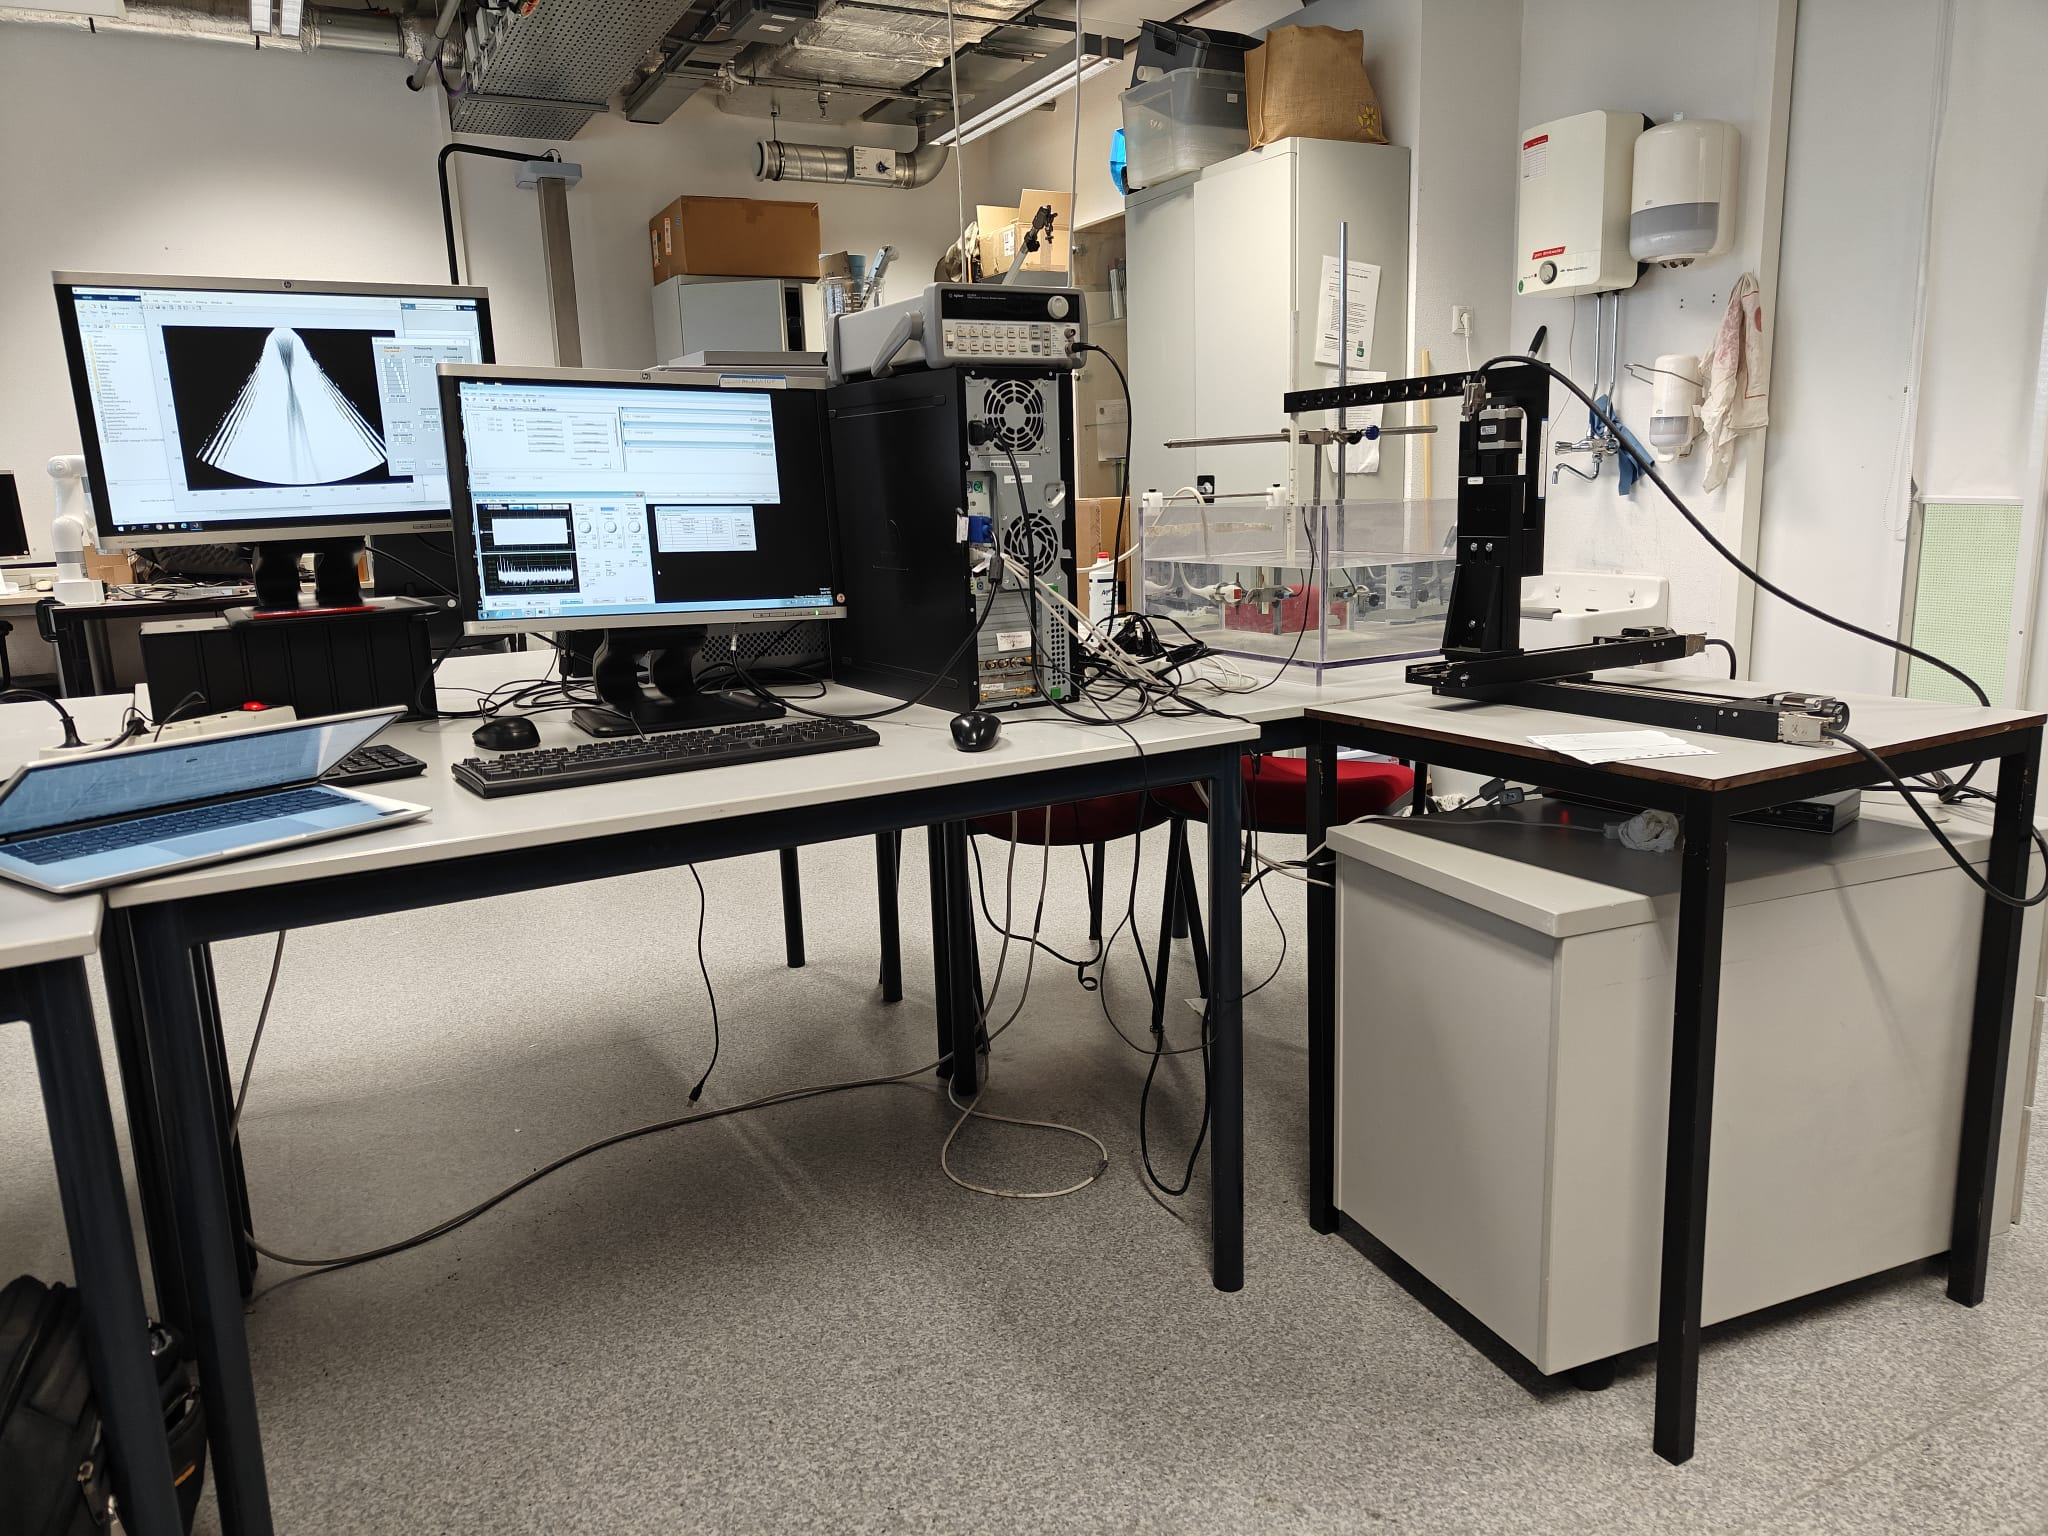
\includegraphics[width=\textwidth]{MI_setup.png}
  \caption{The bench. Left screen: the Verasonics running the measurement sequence. Middle screen:
  the digitizer's Soft Front Panel and the stage control. The digitizer is a card inside the PC
  tower; the water tank and the 3-axis stage are on the bench to the right.}
  \label{fig:setupphoto}
\end{subfigure}\hfill
\begin{subfigure}[b]{0.37\textwidth}
  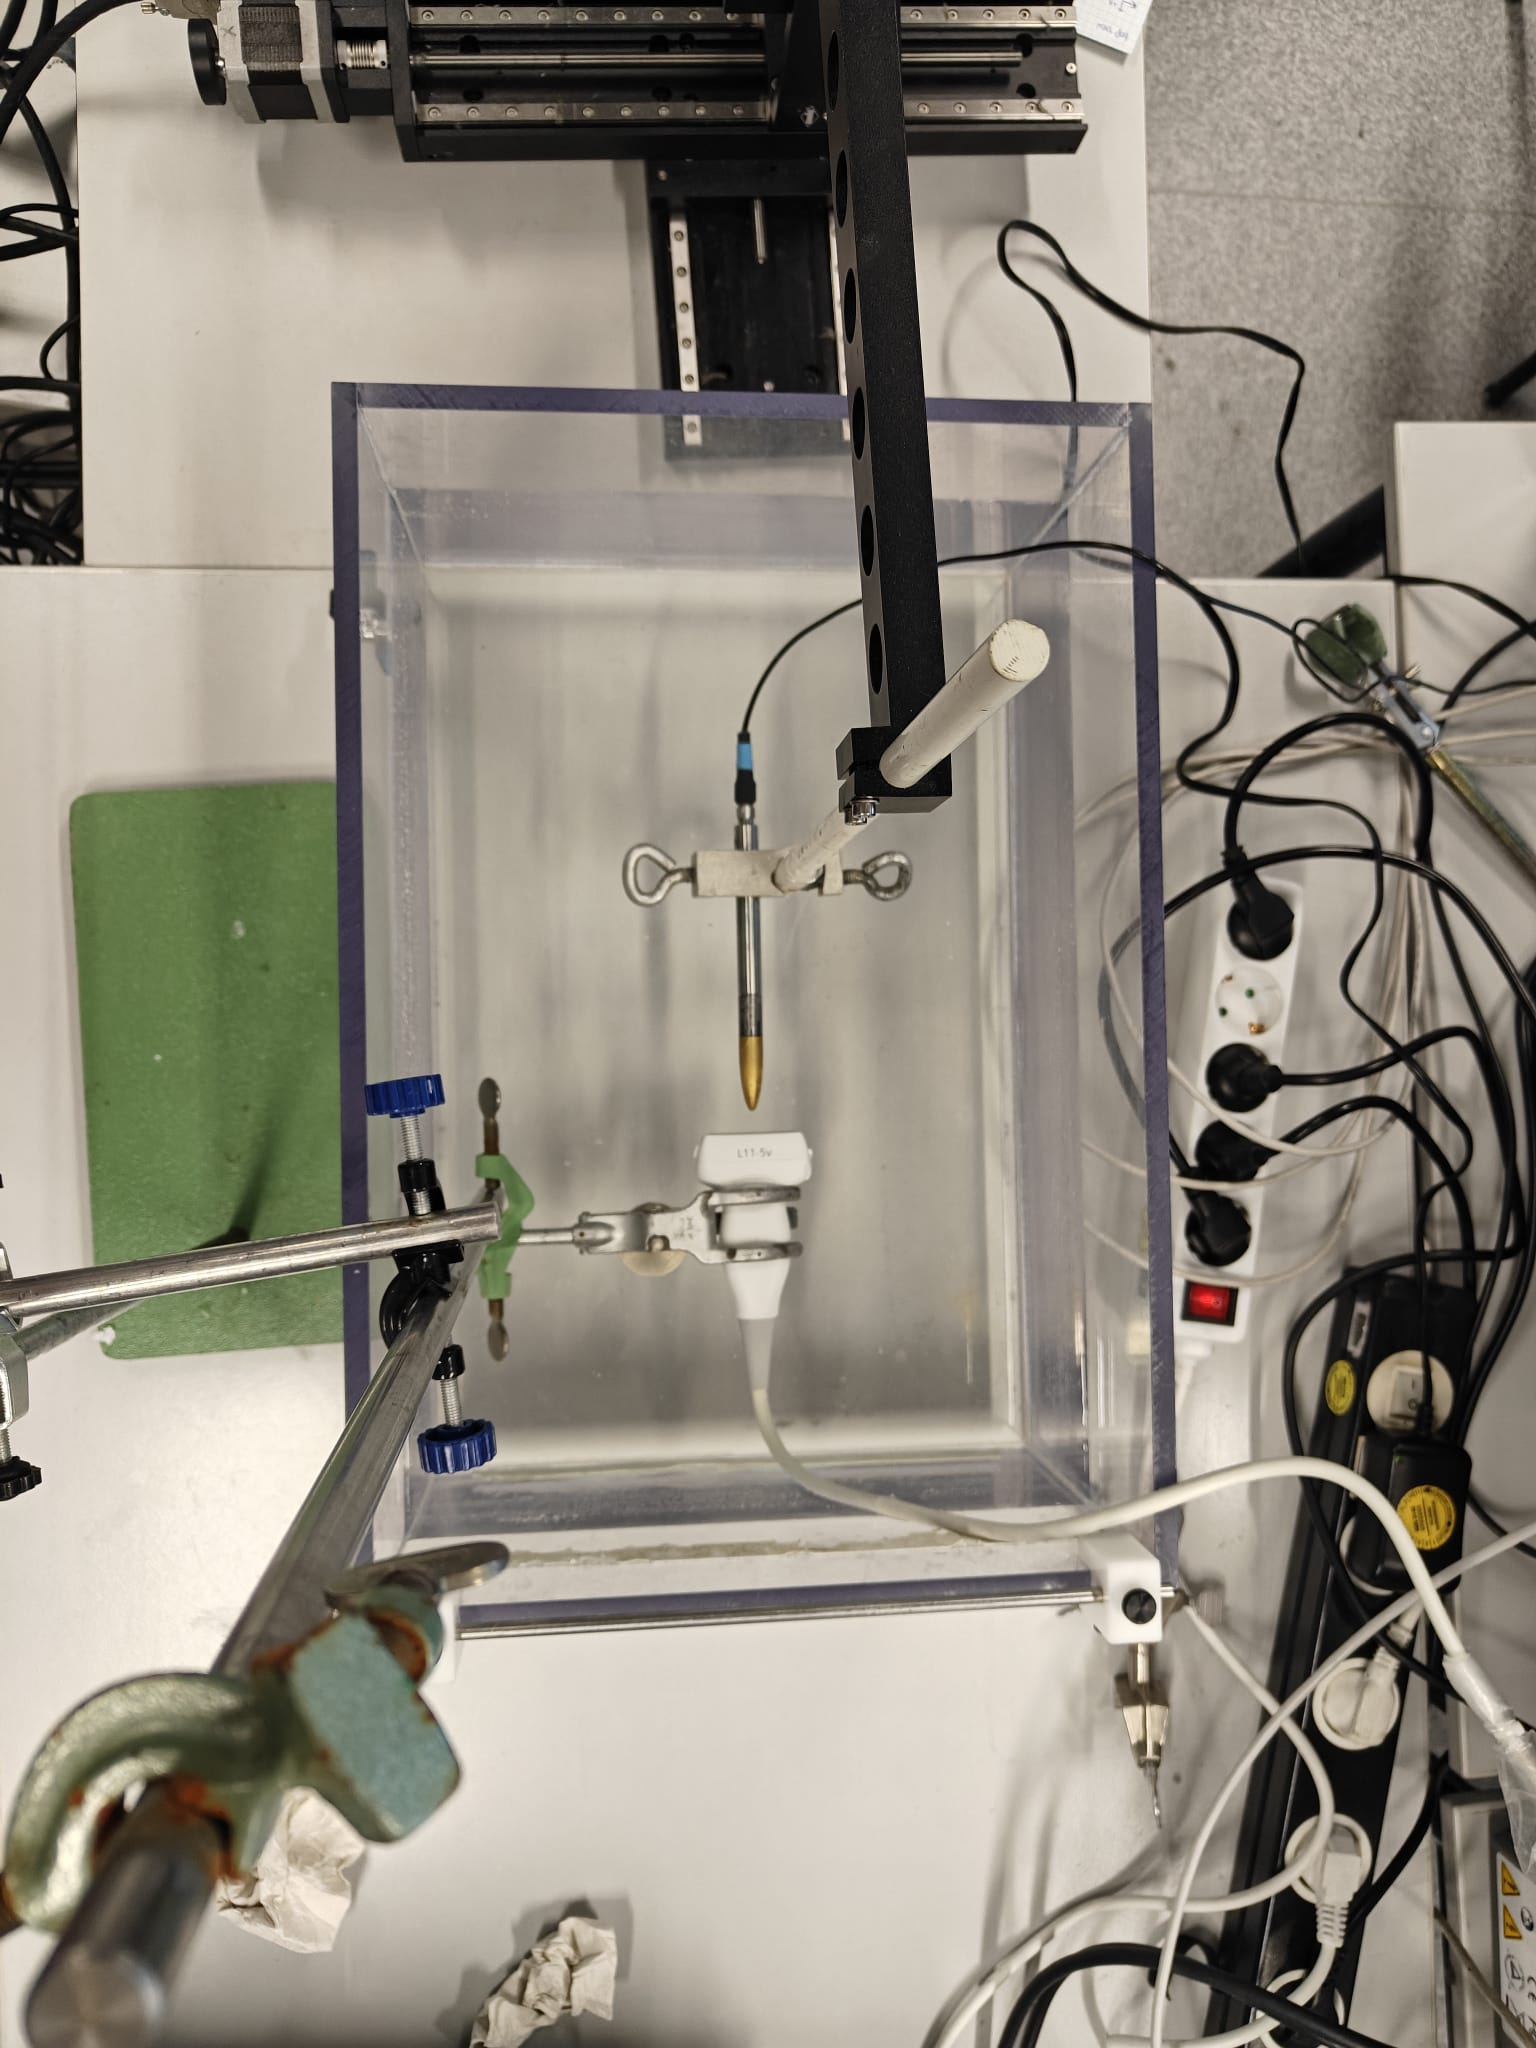
\includegraphics[width=\textwidth]{MI_water_tank.png}
  \caption{The tank. The probe is held in a simple clamp on a laboratory stand; the hydrophone hangs
  from the arm of the 3-axis stage, tip facing the probe. Nothing else is in the water path.}
  \label{fig:tankphoto}
\end{subfigure}
\caption{The measurement setup.}
\label{fig:setup}
\end{figure}

\subsection{The measurement chain}
\begin{description}[style=nextline,leftmargin=1em]
  \item[Hydrophone --- Onda HGL-0400, SN 1037.]
    Capsule hydrophone with a \SI{400}{\micro\metre} nominal sensitive element. The small element is
    what makes it usable at a tight focus: it averages the pressure over its aperture, so a larger
    element under-reads the spatial peak. Open-circuit sensitivity
    $M_c\approx\SI{200}{\nano\volt\per\pascal}$ ($\approx\SI{-254}{\decibel}$ re
    \SI{1}{\volt\per\micro\pascal}) and element capacitance $C_H\approx\SI{12.7}{\pico\farad}$, both
    weakly frequency dependent (Figure~\ref{fig:cal}). Calibrated by Onda on 10-Jun-2024;
    certificates in \texttt{calibration/}.
  \item[Pre-amplifier --- Onda AH-2010-025, SN 1109.]
    Nominal \SI{20}{\decibel} gain, \SI{25}{\mega\hertz} bandwidth, input capacitance
    $C_A=\SI{6.1}{\pico\farad}$, \textbf{output impedance \SI{50}{\ohm}}. Two properties of this box
    dominate the practical side of the measurement: its gain is specified \emph{into a
    \SI{50}{\ohm} load} (\S\ref{sec:impedance}), and its output \textbf{clips at \SI{4}{\volt}
    peak-to-peak into \SI{50}{\ohm}} (\S\ref{sec:clipping}).
  \item[Digitizer --- National Instruments PCI-5112.]
    8-bit, \SI{100}{\mega\hertz} analogue bandwidth, \SI{100}{\mega\sample\per\second} real-time,
    \SIrange{16}{32}{\mega\byte} per channel; a card in the PC, operated through the NI \emph{Scope
    Soft Front Panel} (Scope-SFP 3.8), which writes \texttt{.hws} files. Its input impedance is
    \textbf{software-selectable} between \SI{50}{\ohm} and \SI{1}{\mega\ohm}, which makes the
    impedance cross-check of \S\ref{sec:impedance} a keystroke rather than a cable change.
    \\
    Being \textbf{8-bit} is its one real limitation: only $\approx256$ codes across the vertical
    range, so the range must be set tightly around the signal. Quantisation shows up in the data as
    identical readings at neighbouring positions on a flat part of the field.
  \item[Positioning --- 3-axis motorised translation stage, controlled by OWIsoft.]
    The stage carries the hydrophone; the probe is fixed. All coordinates in this document are stage
    coordinates in \si{\milli\metre}. OWIsoft's meander function --- which drives a predefined grid
    --- is the basis of the ideal measurement of \S\ref{sec:ideal}.
  \item[Tank and mounting.]
    Nothing special is required of the tank: a clear acrylic box large enough to hold the probe, the
    intended stand-off distance and the hydrophone, with room to move the hydrophone past the
    expected field maximum in all three axes. Probe and hydrophone are each held in a simple clamp
    --- the probe on a laboratory stand, the hydrophone on the stage arm (Figure~\ref{fig:tankphoto}).
  \item[Function generator (optional).]
    Useful for an end-to-end electrical check of the acquisition chain: feed a known sine into the
    pre-amplifier input and verify the recorded amplitude and the \SI{50}{\ohm} /
    \SI{1}{\mega\ohm} behaviour before trusting any acoustic number.
\end{description}

\subsection{Water}\label{sec:water}
Ordinary tap water is adequate. Ideally it is degassed and, in any case, left to stand so that
dissolved gas and suspended bubbles settle out --- bubbles on the hydrophone tip or the probe lens
attenuate erratically and cause a low reading that is easily mistaken for a positioning error. There
is no strict protocol; filling the tank the day before and wiping the tip and the lens before
starting covers most of it. Before a session, check both surfaces visually.

\subsection{Reflections}\label{sec:reflections}
The tank walls are strong reflectors --- acrylic against water returns roughly $40\,\%$ of the
incident amplitude, the free surface close to $100\,\%$. Whether that matters depends on the
\textbf{pulse length relative to the round-trip time} to the nearest surface. A short imaging pulse
of a few microseconds arrives long before its own reflection and can simply be gated. A long ARF
push cannot: an \SI{850}{\micro\second} burst occupies over a metre of water path, so in any
bench-scale tank the reflection overlaps the direct field, and the resulting error is
position-dependent --- it distorts the shape of a measured profile, not just its scale.

\good{Line the tank boundaries in the beam path with an acoustic absorber} (rubber tiles, or
open-cell foam as a poorer substitute) whenever long bursts are measured --- at minimum the wall
opposite the probe and the bottom. Whether it is strictly needed in a given tank is testable from
the waveforms already saved: a reflection \textbf{steps} the burst envelope when it arrives and
leaves a \textbf{tail} after the transmit stops, and neither is present if the tank is clean.
\texttt{MakeReportFigures} implements that check. Our own untreated tank turned out to be clean to
better than $1\,\%$, but that result is specific to one tank, probe and geometry and is not a
general licence to skip the absorber.

\subsection{Geometry and the \texttt{Home} convention}\label{sec:home}
The hydrophone is carried by a three-axis OWIS stage; Appendix~\ref{app:owis} is how to drive it,
including where \texttt{Home} is set.
Define, at the start of every session,
\begin{quote}
  \texttt{Home} $=$ the stage coordinate at which the hydrophone tip sits at the \textbf{centre of
  the transducer face},
\end{quote}
and store both \texttt{Home} and the current position \texttt{Pos} in every capture, so that the
derating depth is
\begin{equation}
  z = \lVert \mathtt{Pos} - \mathtt{Home}\rVert .
  \label{eq:depth}
\end{equation}

Derating is exponential in $z$ (Eq.~\ref{eq:derate}); at \SI{2}{\mega\hertz} and \SI{7}{\centi\metre}
a \SI{5}{\milli\metre} error in the assumed origin is already \SI{0.3}{\decibel} on MI and
\SI{0.6}{\decibel} on the intensities. Fixing the origin at the transducer face centre and recording
it in every file removes the ambiguity.

Alignment of the probe to the stage axes need not be perfect, and no effort should be wasted making
it so. The procedure of \S\ref{sec:protocol} \emph{measures around} the misalignment by searching
transversely at every axial station; a small tilt then costs extra search range, not accuracy.

\begin{mistake}
\mistaketitle{using an axis reading as the depth}
The hydrophone is generally not exactly on the beam axis, so a single-axis coordinate difference
under-states the propagation distance. Use the Euclidean distance of Eq.~\ref{eq:depth}.
\end{mistake}

% ======================================================================
\section{Capturing a voltage}\label{sec:voltage}
% ======================================================================
The hydrophone is a capacitive source producing a few hundred \si{\micro\volt} to a few
\si{\milli\volt} per \si{\mega\pascal}. There are two ways to get that onto the digitizer, and a full
characterisation generally needs \textbf{both}, because they cover different parts of the
transmit-voltage range.

\subsection{Chain A: with the pre-amplifier}
The AH-2010 provides \SI{20}{\decibel} of gain, and because its input capacitance
$C_A=\SI{6.1}{\pico\farad}$ is small compared with the hydrophone's own $C_H\approx\SI{12.7}{\pico
\farad}$, only about a third of the signal is lost in the capacitive divider. The resulting system
sensitivity is of order \SI{1.3}{\volt\per\mega\pascal} (Figure~\ref{fig:cal}d). This is the chain to
use at low transmit voltage, and the only one usable when the signal is weak.

\subsection{Chain B: without the pre-amplifier}\label{sec:nopreamp}
Above the clipping ceiling, remove the pre-amplifier and connect the hydrophone directly to the
high-impedance scope input. There is then no gain and --- crucially --- the bare hydrophone is loaded
by the \textbf{entire cable and scope capacitance} $C_\mathrm{load}$ instead of the amplifier's
\SI{6.1}{\pico\farad}. Since $C_\mathrm{load}$ is of order \SI{100}{\pico\farad}, an order of
magnitude above $C_H$, most of the signal is divided away and the sensitivity falls by roughly two
orders of magnitude, to tens of \si{\milli\volt\per\mega\pascal}.

\caveat{$C_\mathrm{load}$ is not a datasheet number, and it dominates the result.} It must be
determined by measurement --- see \S\ref{sec:cloadcal}, which is a mandatory calibration step before
any chain-B result means anything.

\subsection{Oscilloscope input impedance}\label{sec:impedance}
The AH-2010 has a \SI{50}{\ohm} \emph{output} impedance, and its gain --- hence the Onda combined
system sensitivity --- is referenced to a \SI{50}{\ohm} \emph{load}. Terminate that output into a
high-impedance (\SI{1}{\mega\ohm}) scope input instead and the resistive divider disappears: the
scope reads \textbf{twice} the voltage the calibration assumes.

The correction, applied to the measured voltage before anything else, is
\begin{equation}
  V_{50\,\Omega\text{-equiv}} = V_\mathrm{meas}\cdot
  \frac{R_\mathrm{ref}/(R_\mathrm{ref}+R_\mathrm{out})}{R_L/(R_L+R_\mathrm{out})},
  \qquad R_\mathrm{ref}=R_\mathrm{out}=\SI{50}{\ohm},
  \label{eq:loadcorr}
\end{equation}
i.e.\ $\times 0.5$ for $R_L=\SI{1}{\mega\ohm}$ and $\times 1.0$ for $R_L=\SI{50}{\ohm}$. In
\texttt{CalculateSafety.m} this is the \texttt{ScopeImpedance\_Ohm} argument. It applies
\textbf{only with the pre-amplifier} in the chain; without it there is no \SI{50}{\ohm} source and
the loading is capacitive instead (\S\ref{sec:nopreamp}).

\begin{description}[leftmargin=1.2em,style=nextline]
  \item[Rules.]\mbox{}
  \begin{itemize}
    \item \textbf{Measure into \SI{50}{\ohm}} whenever the signal allows it; the calibration then
      applies directly and there is nothing to correct.
    \item \textbf{Record the impedance setting with every single capture.}
    \item \textbf{Verify the $2:1$ ratio once per session} on an unsaturated signal by toggling
      \SI{50}{\ohm} $\leftrightarrow$ \SI{1}{\mega\ohm} without touching anything else. This
      validates the entire resistive part of the calibration in one keystroke.
  \end{itemize}
\end{description}

\begin{mistake}
\mistaketitle{a factor of two, invisible in the waveform}
Forgetting the load correction inflates every pressure and MI by $2\times$ and every intensity by
$4\times$, and nothing about the recorded trace looks wrong. Two independent fingerprints reveal the
scope was on high impedance: the pre-amplifier clipping ceiling appears at $\approx\SI{4.4}{\volt}$
instead of $\approx\SI{2.2}{\volt}$, and the ratio between chains A and B comes out $2\times$ the
expected value. \good{Trust these over the logbook} --- a mis-recorded impedance setting is easy, and
the physical evidence is not.
\end{mistake}

\subsection{Pre-amplifier clipping}\label{sec:clipping}
The AH-2010 output saturates at \SI{4}{\volt} peak-to-peak into \SI{50}{\ohm}, i.e.\
$\approx\SI{2}{\volt}$ peak --- so a chain-A capture is only meaningful below that. Three
consequences:
\begin{enumerate}
  \item \textbf{The pre-amplifier is the ceiling, not the scope.} \caveat{An inline attenuator does
    not help}: it attenuates \emph{after} the stage that is already clipping. Removing the
    pre-amplifier (chain B) does help.
  \item \textbf{Either extrapolate or switch chains.} Since MI is linear in transmit voltage, a
    linear fit through the unsaturated region extrapolates it reliably. Measuring the high-voltage
    points on chain B is better where the sequence permits it, because it captures nonlinear
    saturation and transmit-supply sag, which extrapolation cannot.
  \item \textbf{Overlap the two chains} over several transmit voltages so they can be cross-checked
    against each other, and so $C_\mathrm{load}$ can be determined (\S\ref{sec:cloadcal}).
\end{enumerate}

\begin{mistake}
\mistaketitle{judging clipping from the peak value alone}
Peak voltage versus drive bends over smoothly rather than stopping dead, so a saturating point can
look like an unremarkable data point on a slightly sub-linear curve. \good{Always look at the
waveform}: a clipped trace has visibly flat tops and bottoms (Figure~\ref{fig:clip}a). Discard every
capture that shows them.
\end{mistake}

\begin{figure}[t]
\centering
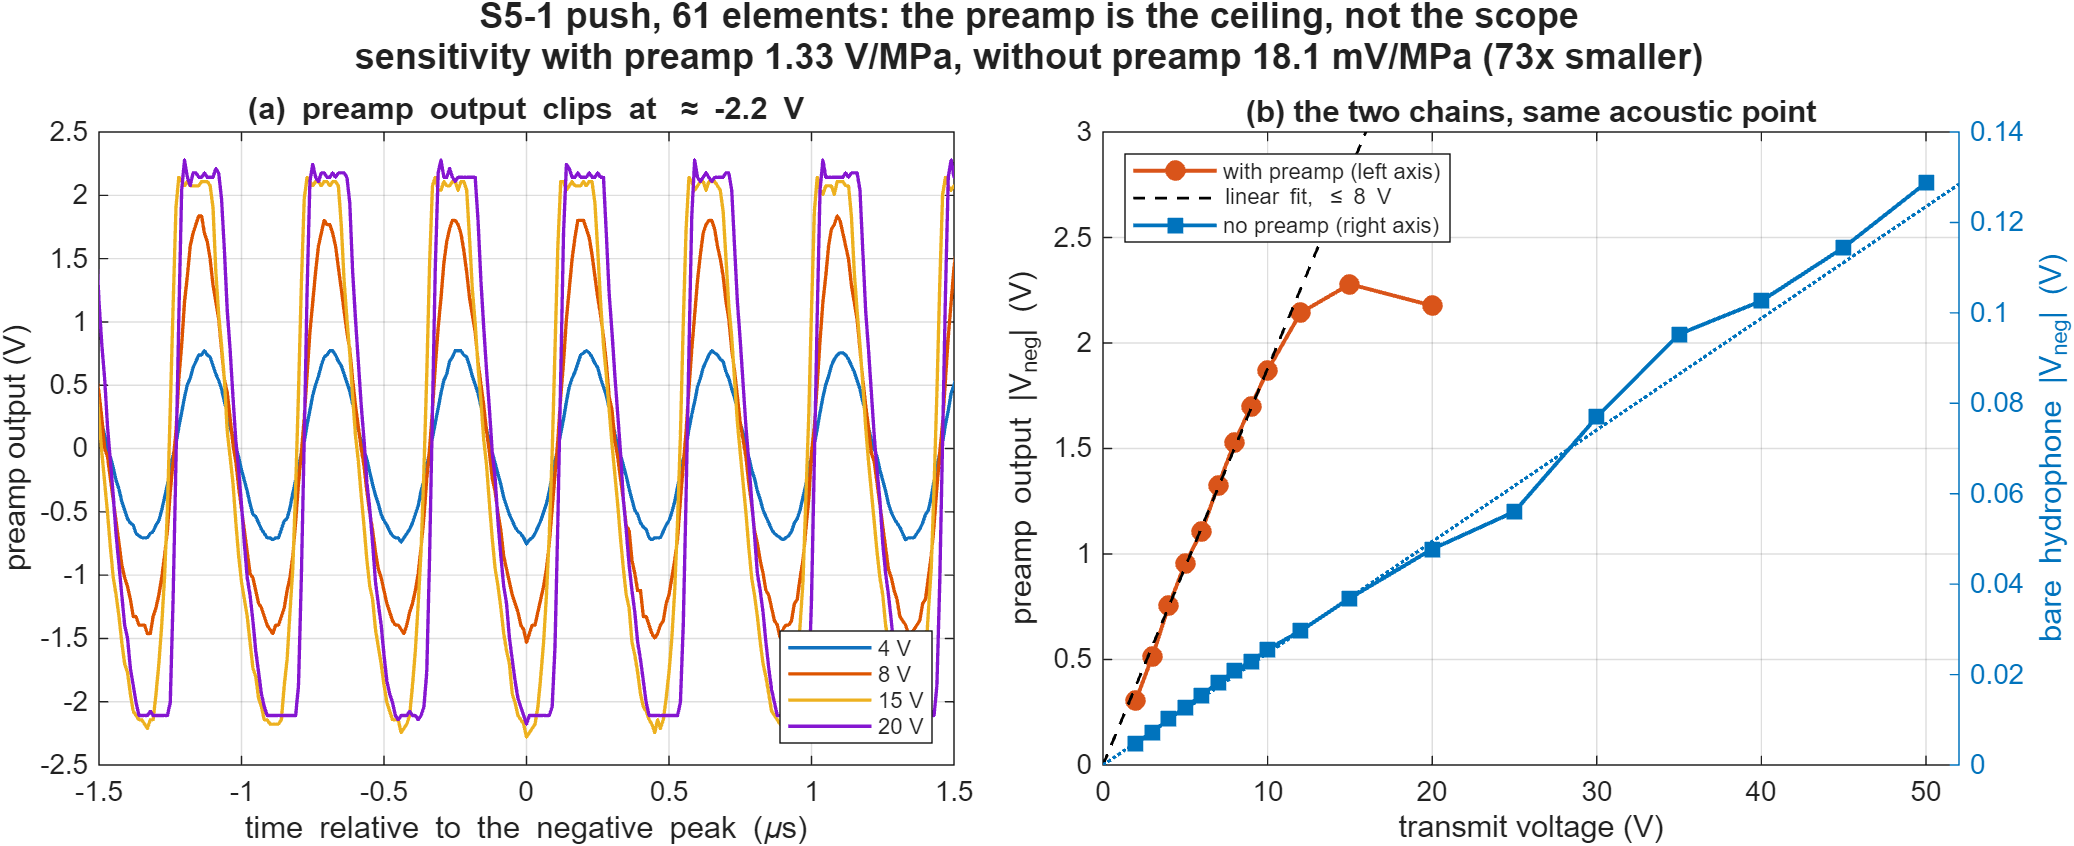
\includegraphics[width=\textwidth]{preamp_clipping.png}
\caption{What clipping looks like, and how the two chains compare. \emph{(a)} Pre-amplifier output at
four transmit voltages, aligned on the negative peak. The lowest trace is a clean (already
nonlinearly distorted) acoustic waveform; the upper two are hard-limited at $\pm\SI{2.2}{\volt}$ and
all amplitude information above that is destroyed. \emph{(b)} Peak negative voltage versus transmit
voltage for both chains at the same acoustic point. Chain A (left axis) departs from its low-voltage
linear fit as it saturates; chain B (right axis) stays linear much further, and the mild flattening
at its top end is genuine acoustic saturation and transmit-supply sag rather than instrument
clipping. Data: S5-1 push, 61 elements.}
\label{fig:clip}
\end{figure}

\subsection{Save the whole waveform}\label{sec:savewaveform}
The scope will display a peak-to-peak number, and it is tempting to record only that. \good{Do not.}
Save the complete digitised record of every capture. Of the quantities in \S\ref{sec:conversion},
only $p_r$ can be recovered from a peak reading; the acoustic working frequency, the pulse duration,
the pulse-intensity integral, the harmonic content, the reflection check of
\S\ref{sec:reflections} and any later re-analysis with a corrected calibration all need the waveform.
Re-measuring is expensive; storage is not.

The Scope-SFP writes \texttt{.hws} (\emph{Hierarchical Waveform Storage}), which is \textbf{HDF5}
underneath and can be read with plain \texttt{h5read} --- no NI drivers required. Samples are stored
as raw 8-bit ADC codes and must be scaled by the stored polynomial $V = c_0 + c_1\cdot\mathrm{raw}$;
\texttt{readHWS.m} does this and also decodes the scope configuration and the free-text note.
Table~\ref{tab:note} is the note to fill in at every capture; it is what lets the analysis
reconstruct depth, aperture and drive without a separate logbook.

\begin{table}[t]
\centering
\small
\caption{The note to write into every \texttt{.hws} capture. \textbf{Required} fields carry
information that cannot be recovered from anywhere else and without which the indices cannot be
computed; the rest is provenance, and never enters the arithmetic.}
\label{tab:note}
\begin{tabular}{llc}
\toprule
Field & Example & Required \\
\midrule
\texttt{Home}             & \texttt{(55.8, 105.84, -17.3) mm} \quad (transducer face centre) & \textbf{yes} \\
\texttt{Pos}              & \texttt{(46.1, 70.84, -17.3) mm} \quad (hydrophone tip)          & \textbf{yes} \\
\texttt{Scope\_impedance} & \texttt{50} \ / \ \texttt{1e6}                                    & \textbf{yes} \\
\midrule
\texttt{Pre-amp}          & \texttt{Yes} \ / \ \texttt{No}                                    & default \\
\texttt{Probe}            & \texttt{S5-1}                                                     & no \\
\texttt{TX\_voltage}      & \texttt{20V}                                                      & no \\
\texttt{Pulse}            & \texttt{normal} \ / \ \texttt{inverted}                           & no \\
\texttt{PushCycles}       & \texttt{1900}                                                     & no \\
\texttt{PushElements}     & \texttt{61}                                                       & no \\
\bottomrule
\end{tabular}
\end{table}

\noindent
Only three fields are load-bearing. \texttt{Home} and \texttt{Pos} give the derating depth
$\lVert\mathtt{Pos}-\mathtt{Home}\rVert$, and \texttt{Scope\_impedance} selects the load correction
of \S\ref{sec:impedance} --- a factor 2 on MI and 4 on the intensities, invisible in the waveform
itself. \texttt{Pre-amp} is the one field with a \emph{default}: if it is absent the pre-amplifier
is taken to have been in the chain, which is the convention the earlier sessions were recorded
under. Write it anyway.

\paragraph{If a required field is missing.} The software does not guess.
\texttt{CaptureConditions.m} resolves the conditions for every capture and, when the note does not
carry one of the three, \textbf{asks for it} --- a menu for the scope impedance, a number for the
depth --- and then labels that value in its output as having been supplied rather than recorded.
Running non-interactively (\texttt{matlab -batch}), where there is nobody to ask, it raises an error
naming the missing field and the argument that supplies it instead. Either way the value can also be
passed directly (\texttt{Depth\_cm}, \texttt{ScopeImpedance\_Ohm}, \texttt{WithPreamp}), which is
the route to take when re-analysing an old capture whose conditions are known from a logbook rather
than from the file.

\begin{mistake}
\mistaketitle{answering the impedance prompt from memory}
The prompt exists to keep an incomplete capture usable, not to make the field optional. An answer
recalled at the end of a long session is exactly the kind of thing that is wrong by a factor of
two, and nothing downstream can catch it. \good{Write the field at acquisition time}, when the
setting is in front of you.
\end{mistake}

\subsection{Scope settings}\label{sec:scopesettings}
\begin{itemize}
  \item \textbf{Real-time sampling at \SI{100}{\mega\sample\per\second}.} \caveat{Never use RIS}
    (random interleaved sampling): any rate above \SI{100}{\mega\sample\per\second} on the 5112 is
    equivalent-time sampling, which reconstructs one waveform from many repetitions. That is valid
    for a repetitive imaging pulse and \textbf{invalid for a single-shot push}. \texttt{readHWS.m}
    warns when it detects the RIS flag.
  \item \textbf{Record length longer than the pulse.} A 1900-cycle push at \SI{2.2}{\mega\hertz}
    lasts \SI{850}{\micro\second}; record \SI{1000}{\micro\second} ($10^5$ samples at
    \SI{100}{\mega\sample\per\second}). A truncated record silently under-reports PII and hence both
    intensities. \texttt{readHWS.m} warns if the record is shorter than the expected pulse.
  \item \textbf{Triggering.} Self-trigger on the hydrophone signal (negative slope, level below the
    smallest expected peak) so the Verasonics can transmit freely with no trigger wire; set a holdoff
    of about one record length to avoid re-triggering on burst ringing. With an external trigger
    instead, set the delay to the time of flight $z/c$ so the window lands on the arrival.
  \item \textbf{Vertical range as tight as the signal allows}, and re-check it after every change of
    transmit voltage. With 8 bits, a range set $4\times$ too wide throws away two bits.
  \item \textbf{DC coupling}; subtract the median of the record as the baseline in post-processing.
\end{itemize}

% ======================================================================
\section{From voltage to MI and the intensities}\label{sec:conversion}
% ======================================================================
All of this is implemented in \texttt{CalculateSafety.m}.

\subsection{Calibration: the loaded sensitivity}\label{sec:calibration}
The Onda certificate for the HGL-0400 is an \textbf{open-circuit} calibration
(\texttt{ELECTRICAL\_LOAD OpenCircuit}): it gives $M_c(f)$, the sensitivity with nothing attached,
and the element capacitance $C_H(f)$. To use it, the load that is actually attached must be added.
With the pre-amplifier that load is its input capacitance $C_A(f)$, giving Onda's ``parallel
circuit'' loaded sensitivity (Eq.~2a of the Onda \emph{HydroCalMethod} note):
\begin{equation}
  M_L(f) = G(f)\; M_c(f)\;\frac{C_H(f)}{C_H(f)+C_A(f)} ,
  \label{eq:senspreamp}
\end{equation}
and without it, the cable-and-scope capacitance takes the place of $C_A$ and there is no gain:
\begin{equation}
  M_L^{\text{no preamp}}(f) = M_c(f)\;\frac{C_H(f)}{C_H(f)+C_\mathrm{load}} .
  \label{eq:sensnopreamp}
\end{equation}

Both $M_c$ and $G$ are frequency dependent, and the tabulated certificates
(\texttt{calibration/}, digested into \texttt{HydrophoneTables.mat}) should be evaluated at the
\emph{measured} $f_\mathrm{awf}$, not at a nominal value. Figure~\ref{fig:cal} shows all of it. Over
\SIrange{1}{20}{\mega\hertz} the hydrophone sensitivity spans about \SI{4}{\decibel} with a sharp dip
near \SI{6}{\mega\hertz}, and the preamp gain droops from \SI{19.95}{\decibel} to
\SI{19}{\decibel}; the combined $M_L$ varies from \SIrange{1.05}{1.6}{\volt\per\mega\pascal} across
that span, though only by a few per cent between neighbouring frequencies in the
\SIrange{2}{5}{\mega\hertz} range.

\begin{mistake}
\mistaketitle{dropping the capacitive divider}
The factor $C_H/(C_H+C_A)\approx0.667$ in Eq.~\ref{eq:senspreamp} is not a refinement. Using a
``simple'' $M_L=G\,M_c$ instead under-reads the pressure by $1.5\times$. Always use the
parallel-circuit form, which is what the code does by default.
\end{mistake}

\begin{mistake}
\mistaketitle{using a nominal sensitivity at a frequency where the calibration has structure}
The \SI{6}{\mega\hertz} dip in Figure~\ref{fig:cal}a is about $20\,\%$ deep and sits exactly where a
harmonic-imaging pulse would land. Interpolate the certificate at the measured $f_\mathrm{awf}$.
\end{mistake}

\begin{figure}[t]
\centering
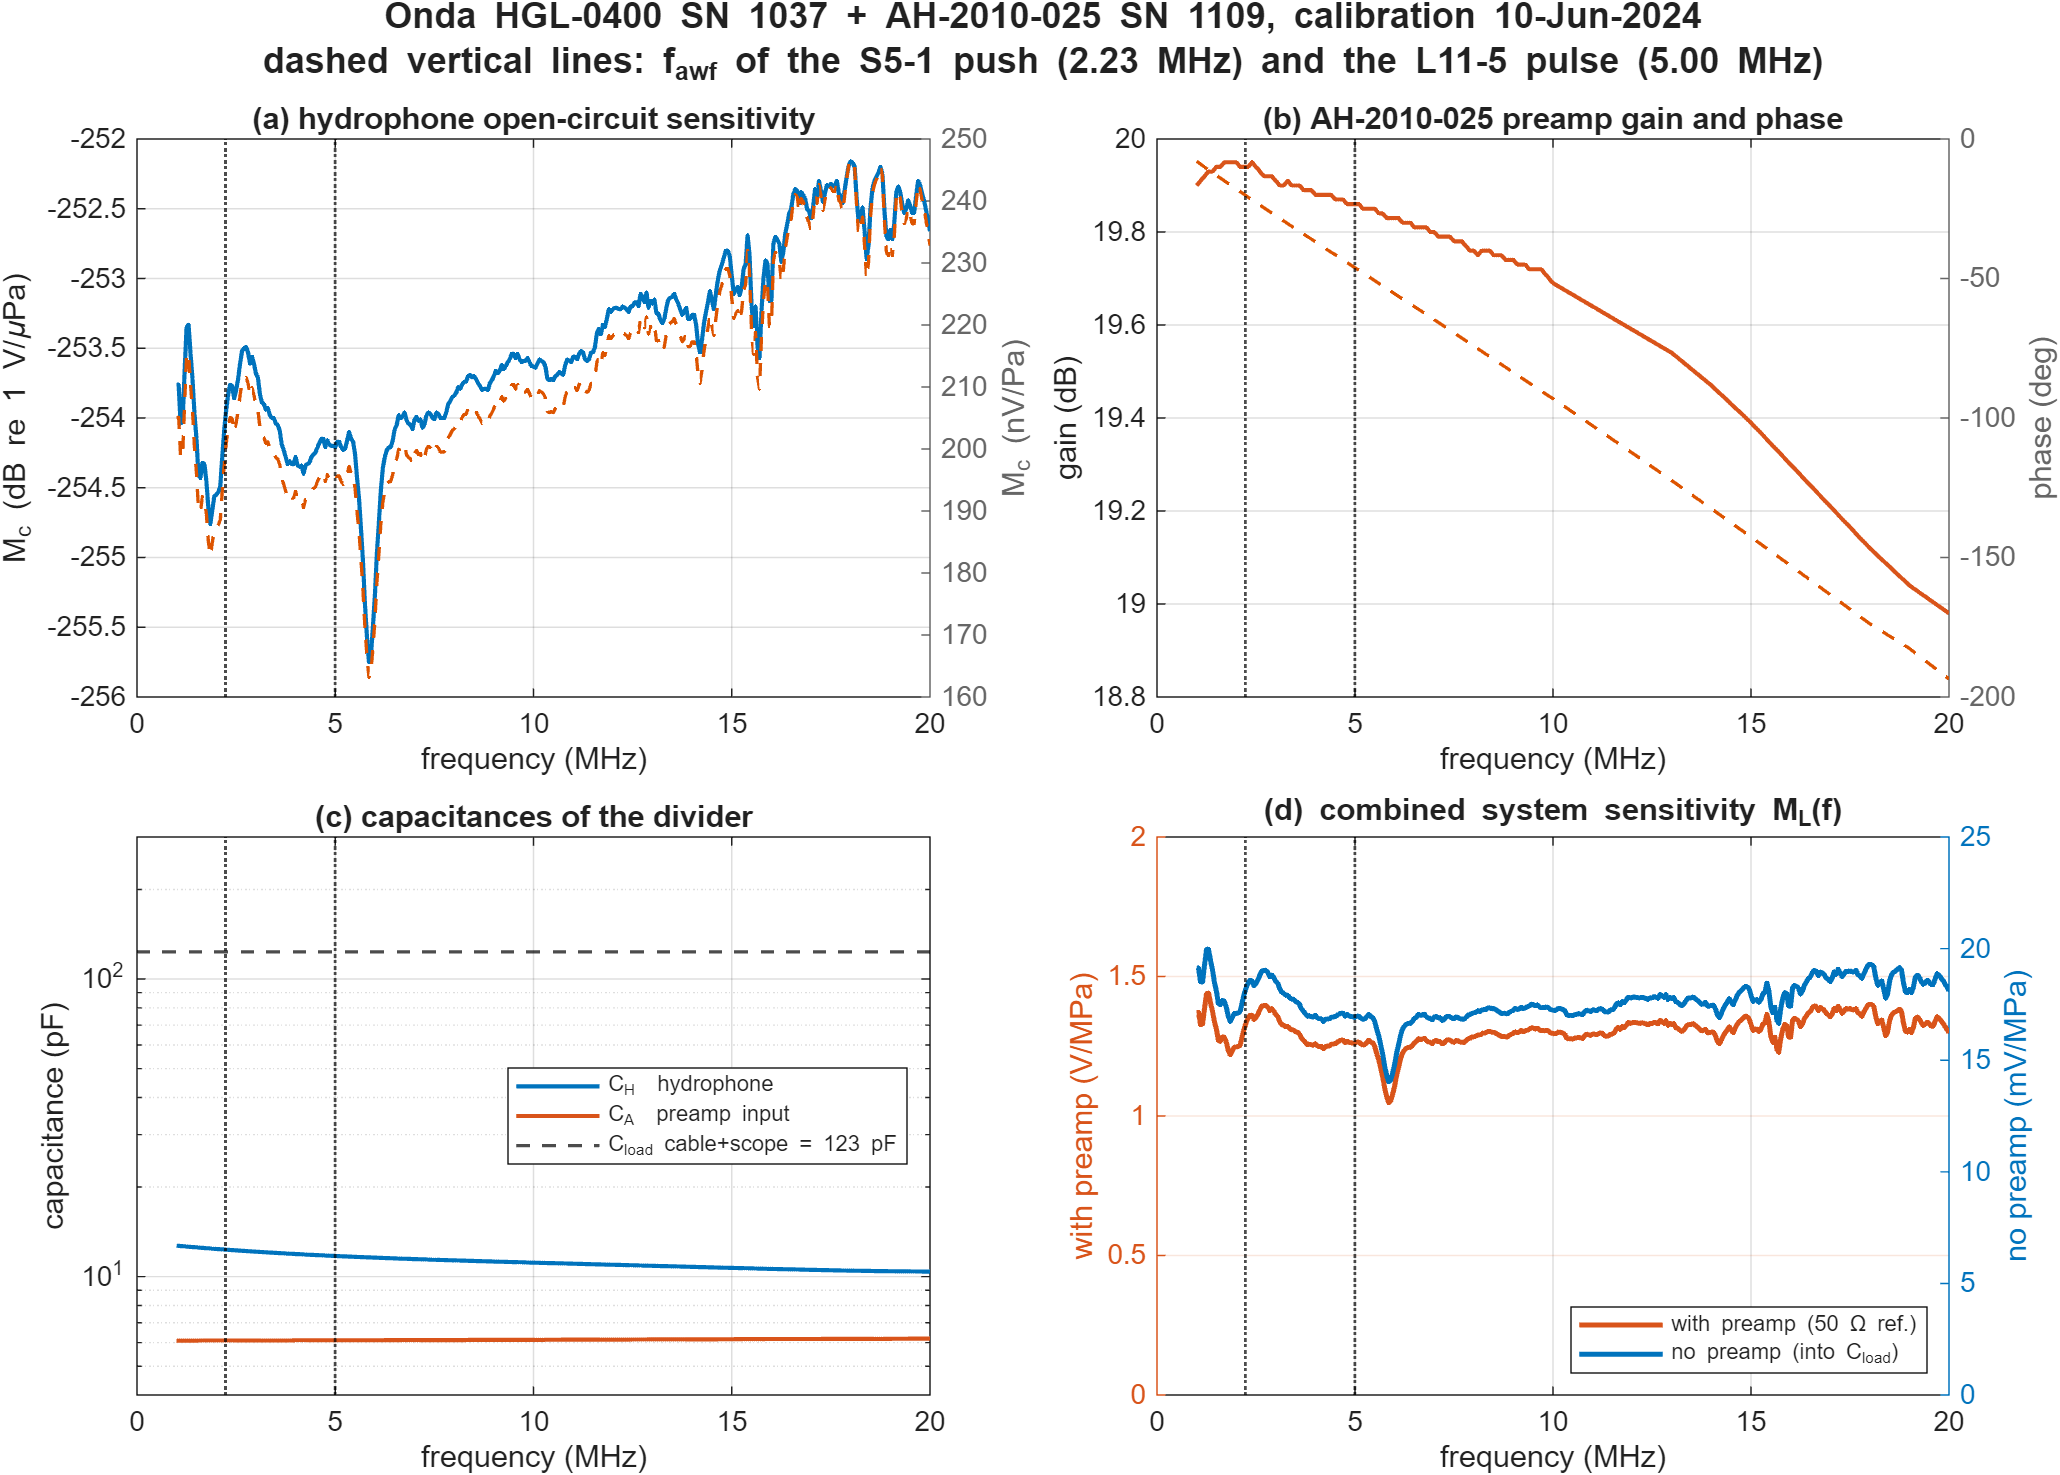
\includegraphics[width=\textwidth]{calibration.png}
\caption{The integrated calibration as a function of frequency. \emph{(a)} Hydrophone open-circuit
sensitivity $M_c$. \emph{(b)} Pre-amplifier gain and phase; the phase matters only for a broadband
deconvolution. \emph{(c)} The three capacitances that set the dividers: $C_H$ (hydrophone), $C_A$
(preamp input, small --- little loss) and $C_\mathrm{load}$ (cable+scope, ten times larger --- most
of the signal lost). \emph{(d)} The combined system sensitivities of Eqs.~\ref{eq:senspreamp} and
\ref{eq:sensnopreamp} --- note the different units on the two axes, a factor $73$ apart. Dotted
vertical lines mark the working frequencies of the two example measurements in \S\ref{sec:results}.}
\label{fig:cal}
\end{figure}

\subsection{Manual calibration of $C_\mathrm{load}$ for the no-preamp chain}\label{sec:cloadcal}
Because $C_\mathrm{load}$ dominates Eq.~\ref{eq:sensnopreamp} and is a property of the specific cable
and scope input rather than a specified value, it has to be measured. The two chains provide the
means: at a fixed acoustic point, and at a drive where the pre-amplifier is unsaturated, their ratio
depends only on known quantities and $C_\mathrm{load}$,
\begin{equation}
  \frac{V_\mathrm{A}}{V_\mathrm{B}} = G\,\frac{C_H+C_\mathrm{load}}{C_H+C_A}
  \quad\Longrightarrow\quad
  C_\mathrm{load} = \frac{V_\mathrm{A}}{V_\mathrm{B}}\cdot\frac{C_H+C_A}{G} - C_H .
  \label{eq:cload}
\end{equation}

\noindent\textbf{Procedure.}
\begin{enumerate}
  \item Park the hydrophone at a point with good signal --- the field maximum is convenient --- and
    do not move the stage, the probe or the tank for the rest of the step.
  \item Choose several transmit voltages spanning the range where chain A is comfortably
    unsaturated (check the waveforms for flat tops).
  \item At each voltage, capture with the pre-amplifier (into \SI{50}{\ohm}), then remove the
    pre-amplifier and capture again (into \SI{1}{\mega\ohm}), changing nothing else.
  \item Compute $V_\mathrm{A}/V_\mathrm{B}$ at each voltage. \good{It must be constant.} Scatter
    beyond a few per cent means something moved, or chain A was already saturating.
  \item Average the ratio over the unsaturated points and solve Eq.~\ref{eq:cload}.
\end{enumerate}

\paragraph{Does this calibration transfer?}
\begin{itemize}
  \item \textbf{Across probes and sequences: yes.} $C_\mathrm{load}$ is a property of the hydrophone
    cable and the scope input --- the electrical side. It contains nothing about the transducer, the
    beam or the drive. Provided the same cable, adapters and scope input are used, the same
    $C_\mathrm{load}$ applies to any probe. (Determined twice, at different probes and different
    frequencies, agreeing to $2\,\%$; see \S\ref{sec:results}. Those two determinations sample
    $C_H(f)$ at \SI{2.2}{} and \SI{5.0}{\mega\hertz}, so their agreement is a genuine check on the
    divider terms $C_H$, $C_A$ and $G$ --- but not on $M_c$, which cancels out of the ratio.)
  \item \textbf{Across frequency: yes, within our band.} The divider
    $C_H(f)/(C_H(f)+C_\mathrm{load})$ depends on frequency only through $C_H$, which falls from
    $\approx\SI{12.7}{\pico\farad}$ to $\approx\SI{10.5}{\pico\farad}$ between \SI{1}{} and
    \SI{20}{\mega\hertz} --- a couple of per cent on the divider. Cable capacitance is essentially
    frequency independent well below the cable's self-resonance.
  \item \caveat{Re-determine it whenever the electrical path changes.} A different cable length, an
    added adapter or BNC tee, or a different scope input all change $C_\mathrm{load}$ directly. It is
    a five-minute measurement; repeat it rather than assume.
\end{itemize}

\subsection{Acoustic working frequency}\label{sec:fawf}
$f_\mathrm{awf}$ enters MI as $1/\sqrt{f}$ and the derating linearly, so it is worth getting right.
Following IEC~62359, take the \textbf{arithmetic centre of the \SI{-6}{\decibel} band of the
fundamental} in the magnitude spectrum of the received waveform (Figure~\ref{fig:wfm}c).

$f_\mathrm{awf}$ is generally \emph{not} the programmed transmit frequency: it is the transmit
spectrum multiplied by the probe's transfer function, and the shift is largest for short, broadband
pulses, which the probe passband pulls toward its own centre.

\begin{mistake}
\mistaketitle{measuring $f_\mathrm{awf}$ at high drive, or over the full band}
As the drive rises, nonlinear propagation builds harmonics, and a wideband centroid then drifts
upward with transmit voltage --- so the ``same'' sequence appears to change frequency. Restrict the
band to the fundamental lobe, and take $f_\mathrm{awf}$ from a \textbf{low-drive} capture.
\end{mistake}

\subsection{Derating}
The regulated quantities describe what a target \emph{in tissue} would experience, but the
measurement is in water, which is essentially lossless. The standard remedy is a fixed
homogeneous-tissue derating of \SI{0.3}{\decibel\per\centi\metre\per\mega\hertz} applied over the
measured propagation distance $z$ of Eq.~\ref{eq:depth}:
\begin{equation}
  p_{.3}(z) = p(z)\cdot 10^{-0.3\,z\,f_\mathrm{awf}/20},
  \qquad z\ \text{in \si{\centi\metre}},\ f_\mathrm{awf}\ \text{in \si{\mega\hertz}} .
  \label{eq:derate}
\end{equation}
Intensities derate with the \emph{square} of that factor, since $I\propto p^2$. Derating is therefore
a depth-dependent tilt on the measured profile, and \textbf{it is what makes the reportable maximum
move} --- see \S\ref{sec:axial}.

\subsection{Pressure, pulse duration and the intensities}
With $M_L$ evaluated at $f_\mathrm{awf}$ and the load correction of Eq.~\ref{eq:loadcorr} applied, the
recorded trace becomes a pressure waveform, $p(t) = V(t)/M_L$, and
\begin{align}
  p_r      &= -\min_t p(t) \quad\text{(peak rarefactional pressure)}, \\
  I(t)     &= \frac{p(t)^2}{\rho c}, \qquad \rho=\SI{1000}{\kilo\gram\per\cubic\metre},\ c=\SI{1500}{\metre\per\second},\\
  \mathrm{PD} &= 1.25\,(t_{90}-t_{10}), \\
  \mathrm{PII} &= \int_{t_{10}}^{t_{90}} I(t)\,\mathrm{d}t ,
\end{align}
where $t_{10}$ and $t_{90}$ are the times at which the cumulative intensity integral reaches
$10\,\%$ and $90\,\%$ of its final value; the $1.25$ factor is the convention that converts that
$10$--$90\,\%$ span into an equivalent pulse duration. MI, $I_\mathrm{sppa.3}$ and
$I_\mathrm{spta.3}$ then follow from Eqs.~\ref{eq:mi}--\ref{eq:ispta}, with $\mathrm{PII}_{.3}$ the
PII computed from the derated pressure. Figure~\ref{fig:wfm} shows every one of these read off a
single capture.

\begin{mistake}
\mistaketitle{taking $p_r$ as half the peak-to-peak}
At the pressures involved, propagation is nonlinear and the waveform is asymmetric --- compressional
peaks are sharper and taller than the rarefactional troughs. MI uses the \emph{rarefactional} half
specifically. Take the minimum of the trace, never $V_\mathrm{pp}/2$.
\end{mistake}

\begin{mistake}
\mistaketitle{using the line PRF for $I_\mathrm{spta}$}
The PRF in Eq.~\ref{eq:ispta} is the \textbf{local} one: how often \emph{that point in space} is
insonified. For a scanned sequence that is the frame rate, not the line rate --- a sequence firing 71
lines at \SI{270}{\micro\second} PRI insonifies any given point once per \SI{19.2}{\milli\second}
frame, i.e.\ at \SI{52}{\hertz} and not \SI{3.7}{\kilo\hertz}, a factor 71. For a burst-mode push,
use the true duty cycle over the repeat period, including the off time.
\end{mistake}

\begin{figure}[t]
\centering
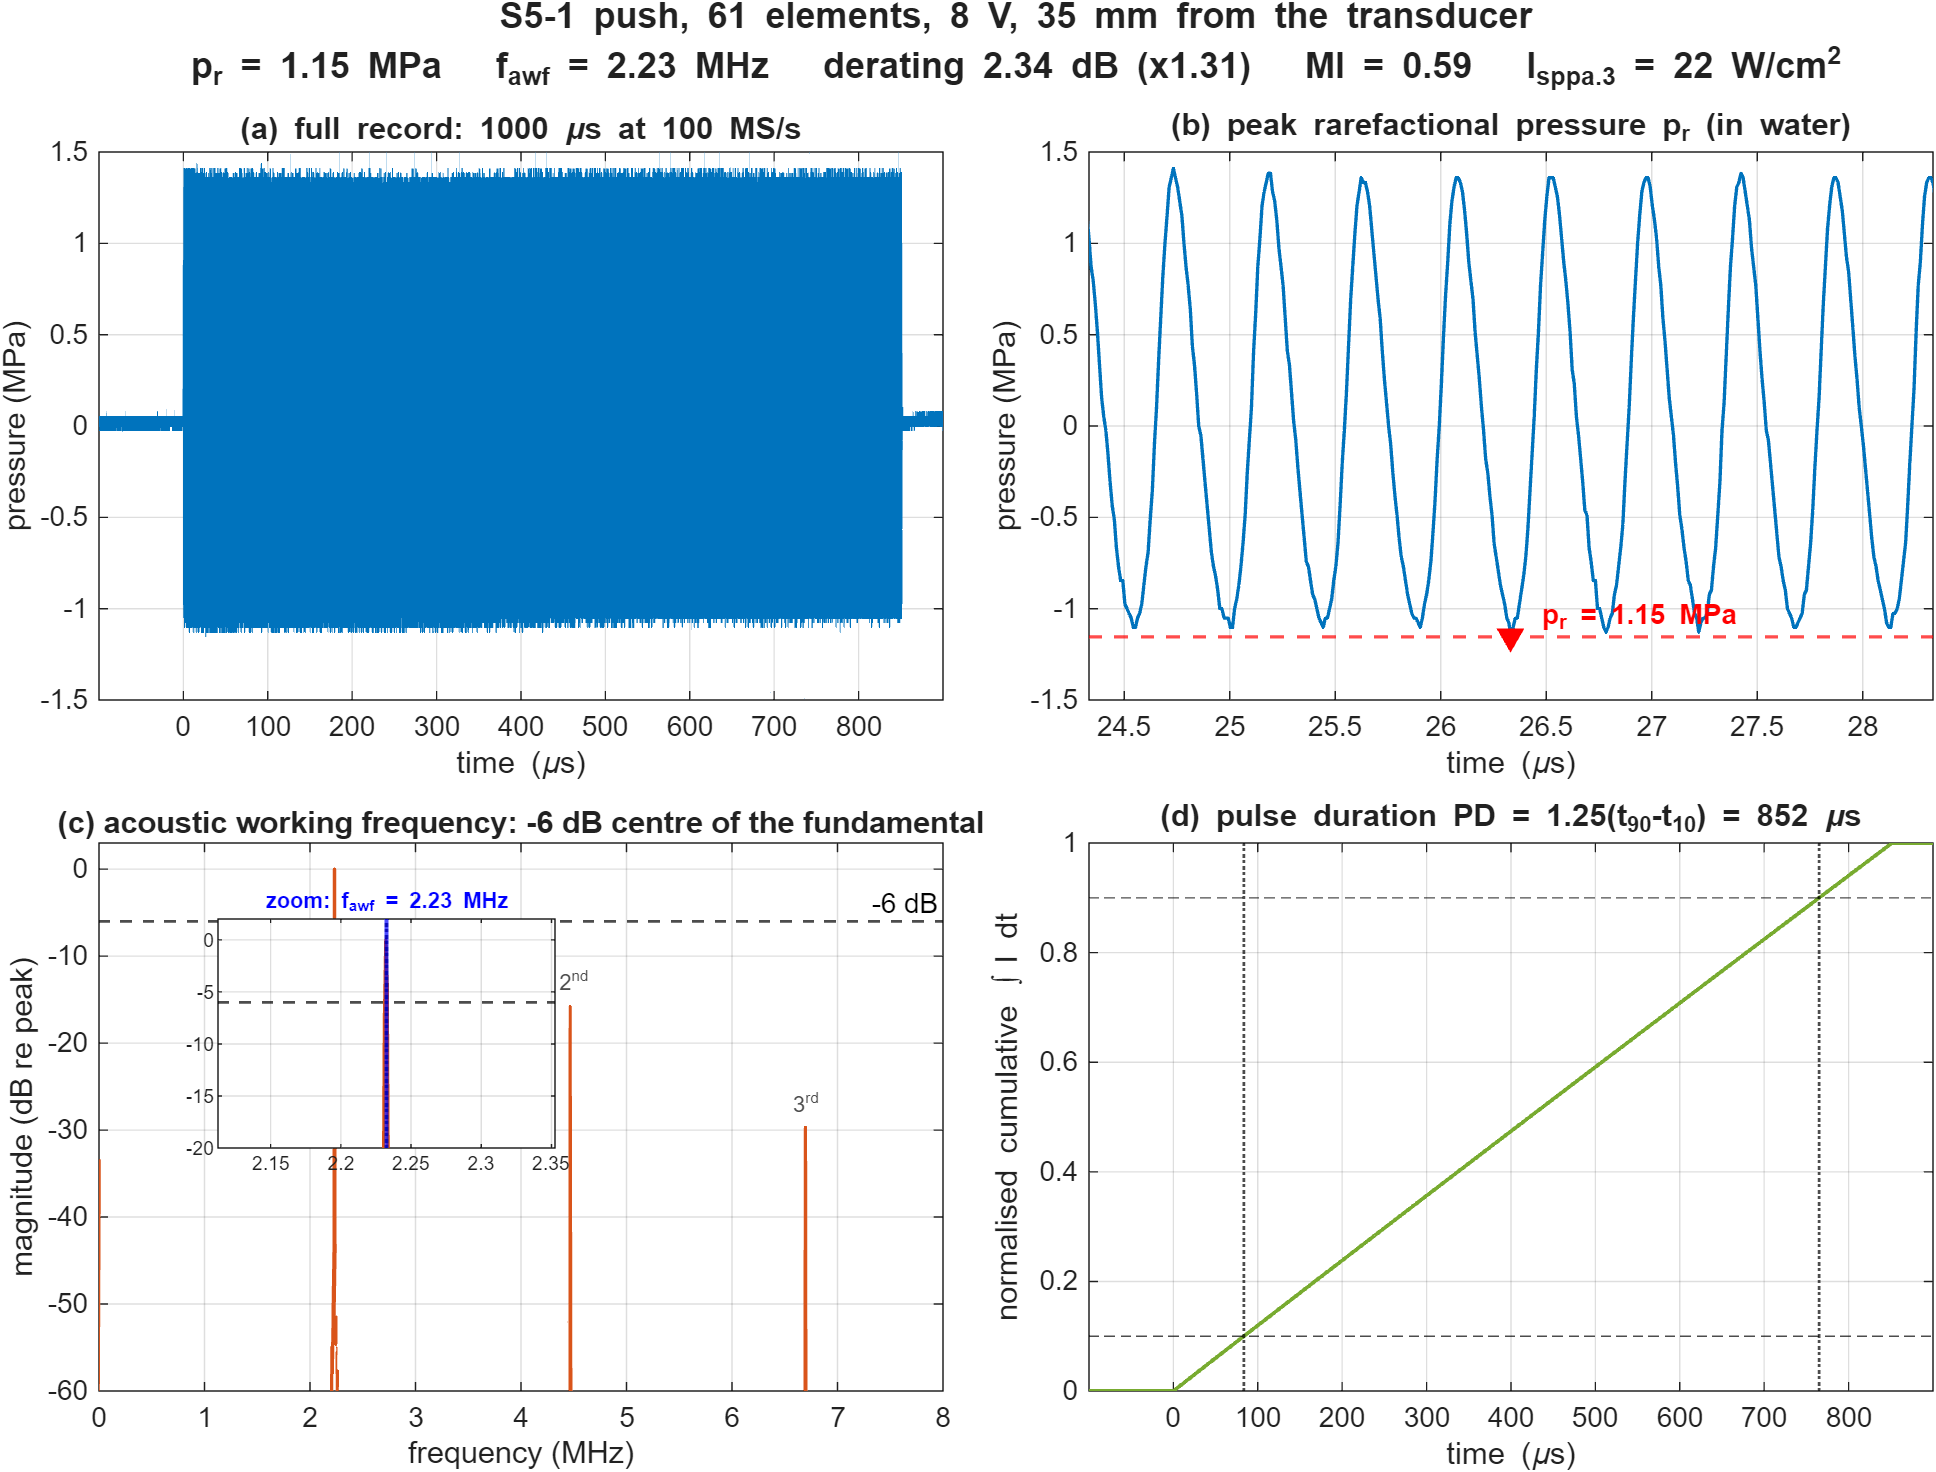
\includegraphics[width=\textwidth]{waveform_metrics.png}
\caption{Everything extracted from one saved waveform (S5-1 push, 61 elements, \SI{8}{\volt},
\SI{35}{\milli\metre} from the transducer). \emph{(a)} The full \SI{1000}{\micro\second} record; the
1900-cycle burst fills \SI{850}{\micro\second} of it. \emph{(b)} A few cycles around the negative
peak; the waveform is visibly asymmetric --- peaks at $+\SI{1.40}{\mega\pascal}$, troughs only at
$-\SI{1.15}{\mega\pascal}$ --- which is nonlinear propagation. \emph{(c)} Magnitude spectrum: the
\SI{-6}{\decibel} centre of the fundamental gives $f_\mathrm{awf}$ (inset), with second and third
harmonics at $-16$ and \SI{-30}{\decibel}. \emph{(d)} Cumulative intensity integral, from which the
pulse duration and PII follow.}
\label{fig:wfm}
\end{figure}

\subsection{Refinements that are usually not needed}\label{sec:broadband}
Two corrections are available and both are small, in the direction of \emph{increasing} the reported
values:
\begin{itemize}
  \item \textbf{Spatial averaging.} The \SI{400}{\micro\metre} element averages the pressure over its
    face and so under-reads a tight focus. A jinc focal-plane model
    (\texttt{spatialAvgFactor.m}) gives a correction of a few per cent for our geometries.
  \item \textbf{Broadband deconvolution.} Instead of dividing by $M_L(f_\mathrm{awf})$, deconvolve
    the full spectrum with $M_L(f)$ including the amplifier phase
    (\texttt{voltageToPressureBroadband.m}). This changes MI by a few per cent, more at high drive
    where harmonics matter.
\end{itemize}
The single-frequency method is the default because it is what the standard prescribes and what
reference values use. Since both corrections raise the reported values, leaving them out is
\emph{not} conservative --- quote them as an uncertainty rather than ignoring them.

% ======================================================================
\section{Measurement protocol}\label{sec:protocol}
% ======================================================================
% ----------------------------------------------------------------------
%  Figure: the measurement on one page.
%  Left column  = the steps, in order.
%  Right column = the point in each step that is easiest to get wrong.
%  Included from main.tex; needs tikz + the pstep/pwatch styles defined there.
%  (They are NOT called step/watch: /tikz/step is a built-in TikZ key.)
% ----------------------------------------------------------------------
\begin{figure}[p]
\centering
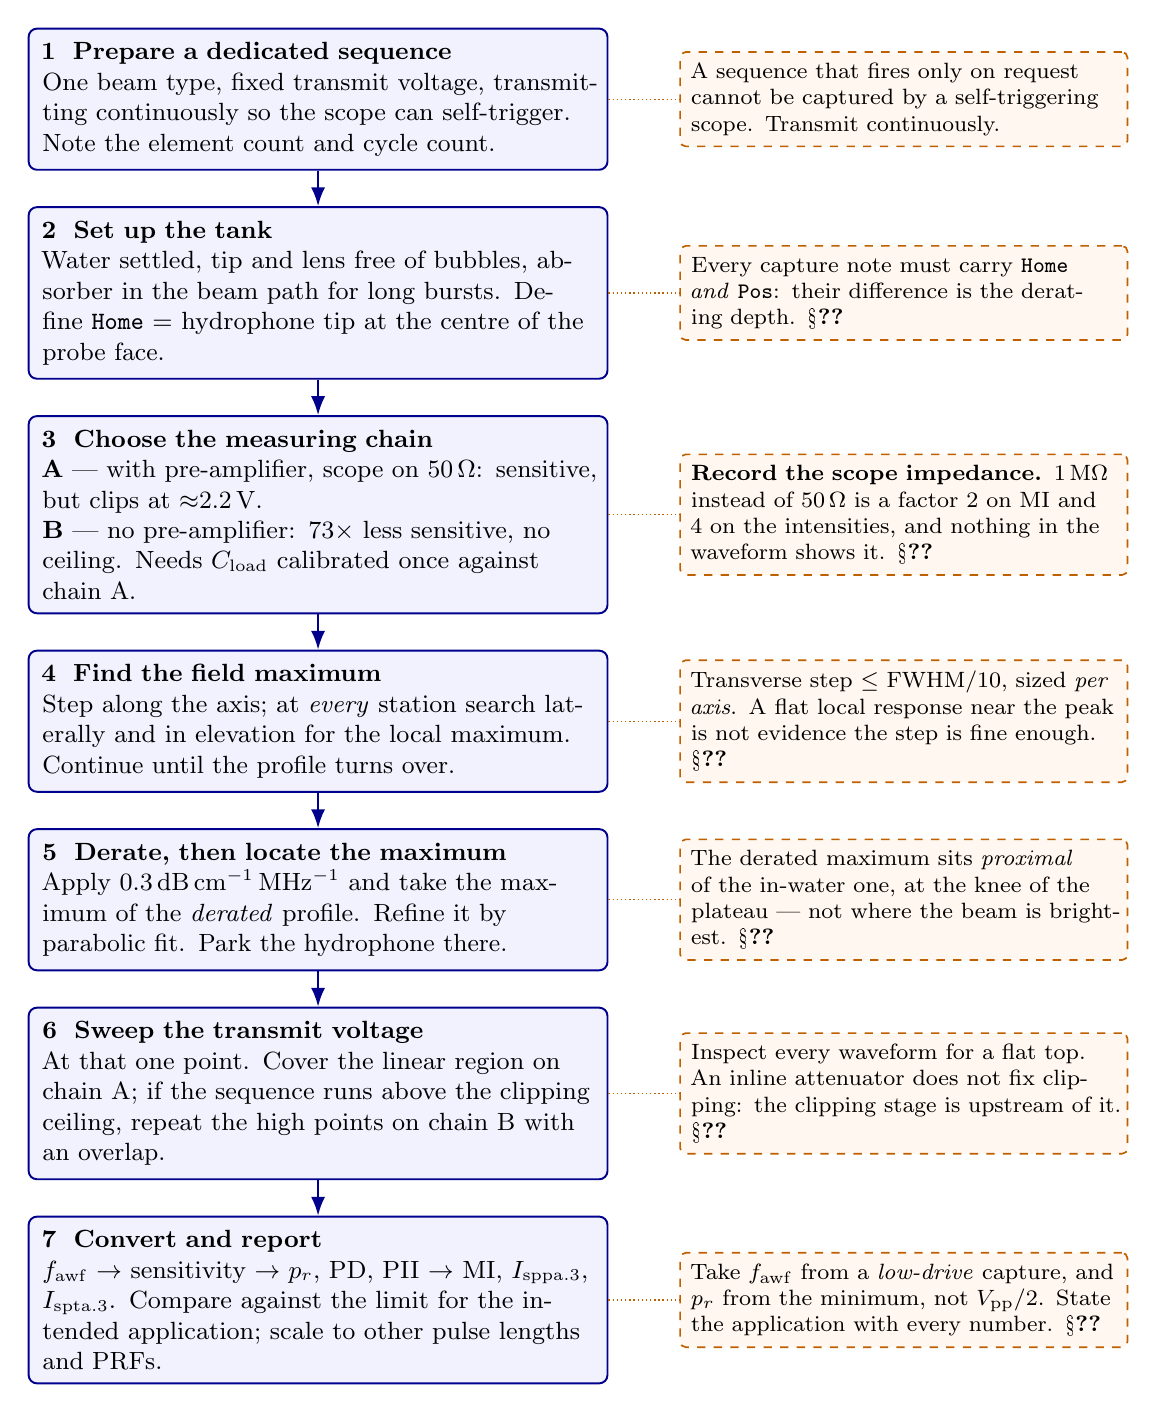
\begin{tikzpicture}[node distance=4.5mm]

% ---------------- the steps -------------------------------------------
\node[pstep] (s1)
  {\textbf{1 \ Prepare a dedicated sequence}\\
   One beam type, fixed transmit voltage, transmitting continuously so the scope
   can self-trigger. Note the element count and cycle count.};

\node[pstep, below=of s1] (s2)
  {\textbf{2 \ Set up the tank}\\
   Water settled, tip and lens free of bubbles, absorber in the beam path for long
   bursts. Define \texttt{Home} $=$ hydrophone tip at the centre of the probe face.};

\node[pstep, below=of s2] (s3)
  {\textbf{3 \ Choose the measuring chain}\\
   \textbf{A} --- with pre-amplifier, scope on \SI{50}{\ohm}: sensitive, but clips
   at $\approx$\SI{2.2}{\volt}.\\
   \textbf{B} --- no pre-amplifier: $73\times$ less sensitive, no ceiling. Needs
   $C_\mathrm{load}$ calibrated once against chain~A.};

\node[pstep, below=of s3] (s4)
  {\textbf{4 \ Find the field maximum}\\
   Step along the axis; at \emph{every} station search laterally and in elevation for
   the local maximum. Continue until the profile turns over.};

\node[pstep, below=of s4] (s5)
  {\textbf{5 \ Derate, then locate the maximum}\\
   Apply \SI{0.3}{\decibel\per\centi\metre\per\mega\hertz} and take the maximum of
   the \emph{derated} profile. Refine it by parabolic fit. Park the hydrophone there.};

\node[pstep, below=of s5] (s6)
  {\textbf{6 \ Sweep the transmit voltage}\\
   At that one point. Cover the linear region on chain~A; if the sequence runs above
   the clipping ceiling, repeat the high points on chain~B with an overlap.};

\node[pstep, below=of s6] (s7)
  {\textbf{7 \ Convert and report}\\
   $f_\mathrm{awf}\rightarrow$ sensitivity $\rightarrow p_r$, PD, PII $\rightarrow$
   MI, $I_\mathrm{sppa.3}$, $I_\mathrm{spta.3}$. Compare against the limit for the
   intended application; scale to other pulse lengths and PRFs.};

\foreach \i/\j in {s1/s2, s2/s3, s3/s4, s4/s5, s5/s6, s6/s7}
  \draw[flow] (\i) -- (\j);

% ---------------- what to watch, one per step -------------------------
\node[pwatch, right=9mm of s1] (w1)
  {A sequence that fires only on request cannot be captured by a self-triggering
   scope. Transmit continuously.};

\node[pwatch, right=9mm of s2] (w2)
  {Every capture note must carry \texttt{Home} \emph{and} \texttt{Pos}: their
   difference is the derating depth. \S\ref{sec:home}};

\node[pwatch, right=9mm of s3] (w3)
  {\textbf{Record the scope impedance.} \SI{1}{\mega\ohm} instead of
   \SI{50}{\ohm} is a factor 2 on MI and 4 on the intensities, and nothing in the
   waveform shows it. \S\ref{sec:impedance}};

\node[pwatch, right=9mm of s4] (w4)
  {Transverse step $\le\mathrm{FWHM}/10$, sized \emph{per axis}. A flat local
   response near the peak is not evidence the step is fine enough.
   \S\ref{sec:stepsize}};

\node[pwatch, right=9mm of s5] (w5)
  {The derated maximum sits \emph{proximal} of the in-water one, at the knee of the
   plateau --- not where the beam is brightest. \S\ref{sec:axial}};

\node[pwatch, right=9mm of s6] (w6)
  {Inspect every waveform for a flat top. An inline attenuator does not fix
   clipping: the clipping stage is upstream of it. \S\ref{sec:clipping}};

\node[pwatch, right=9mm of s7] (w7)
  {Take $f_\mathrm{awf}$ from a \emph{low-drive} capture, and $p_r$ from the
   minimum, not $V_\mathrm{pp}/2$. State the application with every number.
   \S\ref{sec:fawf}};

\foreach \i in {1,...,7}
  \draw[hint] (s\i) -- (w\i);

\end{tikzpicture}
\caption{The measurement in seven steps (blue), each with the thing most easily got wrong in it
(orange). Steps 4 and 5 are the ones that consume the time; step 3 is the one that silently
invalidates everything downstream if the scope impedance is not recorded.}
\label{fig:flow}
\end{figure}



\subsection{Step 1 --- prepare a dedicated sequence}
Do not measure the clinical sequence directly. Write a variant that transmits \textbf{a single,
centred, non-steered beam}, repeated continuously at a convenient rate. The beam itself can be
whatever the sequence uses --- tightly focused, diverging, or anything in between --- but it must be
one beam, on the array centre, unsteered:
\begin{itemize}
  \item \textbf{Centred and unsteered}, so the beam axis is nearly normal to the probe face; the
    axial sweep is then a straight line in stage coordinates and the transverse search stays small.
  \item \textbf{A single beam}, so the hydrophone is not sampling a different transmit on every
    trigger. Under a scanned sequence each line is seen once per frame, which mixes geometries and
    makes the local PRF ambiguous.
  \item \textbf{Repeated continuously}, so the scope can free-run on its own trigger.
\end{itemize}
Keep the transmit \emph{waveform} --- frequency, cycles, apodisation, aperture, focal depth ---
identical to the sequence being certified; those are what set the field. The PRF may differ, since
$I_\mathrm{spta}$ is scaled analytically afterwards (\S\ref{sec:scaling}).

\subsection{Step 2 --- set up and check}
\begin{enumerate}
  \item Mount probe and hydrophone facing each other, wipe both surfaces, and check for bubbles.
  \item Define \texttt{Home} at the transducer face centre (\S\ref{sec:home}).
  \item Verify the $2:1$ impedance ratio (\S\ref{sec:impedance}).
  \item Run the reflection check of \S\ref{sec:reflections} if the pulse is long, and add absorber if
    the burst envelope is not flat.
  \item Determine $C_\mathrm{load}$ (\S\ref{sec:cloadcal}) if chain B will be used.
  \item Capture at low drive and confirm $f_\mathrm{awf}$ (\S\ref{sec:fawf}).
\end{enumerate}

\subsection{Step 3 --- find the maximum of the derated field}\label{sec:axial}
The regulated quantity is the maximum of the \textbf{derated} field, and \good{its location is not
known until the data have been analysed.} Three effects displace it from the nominal focus:
diffraction (focal shift, proximal), nonlinear propagation (further proximal), and derating, which
grows with depth and therefore \textbf{always pulls the maximum proximal}. Probe--hydrophone
misalignment displaces it laterally and in elevation. Hence:

\begin{enumerate}
  \item \textbf{Start conservatively shallow.} Use a field simulation to bracket where the in-water
    focus should be, then \textbf{begin proximal of it}, because the derated maximum is on that side.
  \item \textbf{Step along the axis.} A uniform \SI{3}{\milli\metre} step is a reasonable default. A
    two-stage alternative is a coarse \SI{5}{\milli\metre} map followed by a \SI{2}{\milli\metre}
    refinement within $\pm\SI{10}{\milli\metre}$ of the observed maximum. As a rule of thumb the
    $-6$\,dB depth of focus is $\approx 7.1\,F_\#^2\lambda$; take a step of roughly a tenth of that.
  \item \textbf{At every axial station, search transversely.} Move in lateral and elevation to find
    the local maximum of $|V_\mathrm{neg}|$ before saving. This is what corrects the
    probe--hydrophone misalignment, and \good{the step size here is the single most
    under-estimated parameter in the whole measurement} --- see \S\ref{sec:stepsize}. Work in two
    passes: a coarse pass at $\approx\mathrm{FWHM}/3$ over $\pm1$ FWHM to locate the lobe, then a
    \textbf{fine pass at $\approx\mathrm{FWHM}/10$}, which for our probes means
    \SIrange{0.1}{0.2}{\milli\metre}.
  \item \textbf{Save only the local peak waveform, with its coordinates}, in the note format of
    Table~\ref{tab:note}. One sweep then serves MI and both intensities.
  \item \textbf{Continue until the profile clearly turns over} and stays down for several stations,
    so the maximum is genuinely bracketed.
  \item \textbf{Analyse before concluding.} Apply the derating and take the maximum of the derated
    profile --- not of the raw one --- then refine it by parabolic interpolation and check that the
    axial step was fine enough (\S\ref{sec:stepsize}).
\end{enumerate}

\begin{mistake}
\mistaketitle{stopping the sweep at the nominal focus}
Because derating tilts the profile proximal, the derated maximum can sit well shallower than the
in-water focus --- particularly for a deep focus, where the in-water field is a long plateau and the
derating gradient across it is large. A sweep that stops at, or starts at, the nominal focus can miss
it entirely and under-report MI substantially.
\end{mistake}

\begin{mistake}
\mistaketitle{skipping the transverse search}
An uncorrected elevation offset produces a \emph{constant multiplicative} under-read: the shape of
every curve is right, the slope of MI against transmit voltage is right, and only the absolute value
is wrong. \good{A constant factor across a voltage sweep is a positioning error, not a calibration
error} --- and if only one location is ever measured, the two are indistinguishable.
\end{mistake}

\begin{figure}[t]
\centering
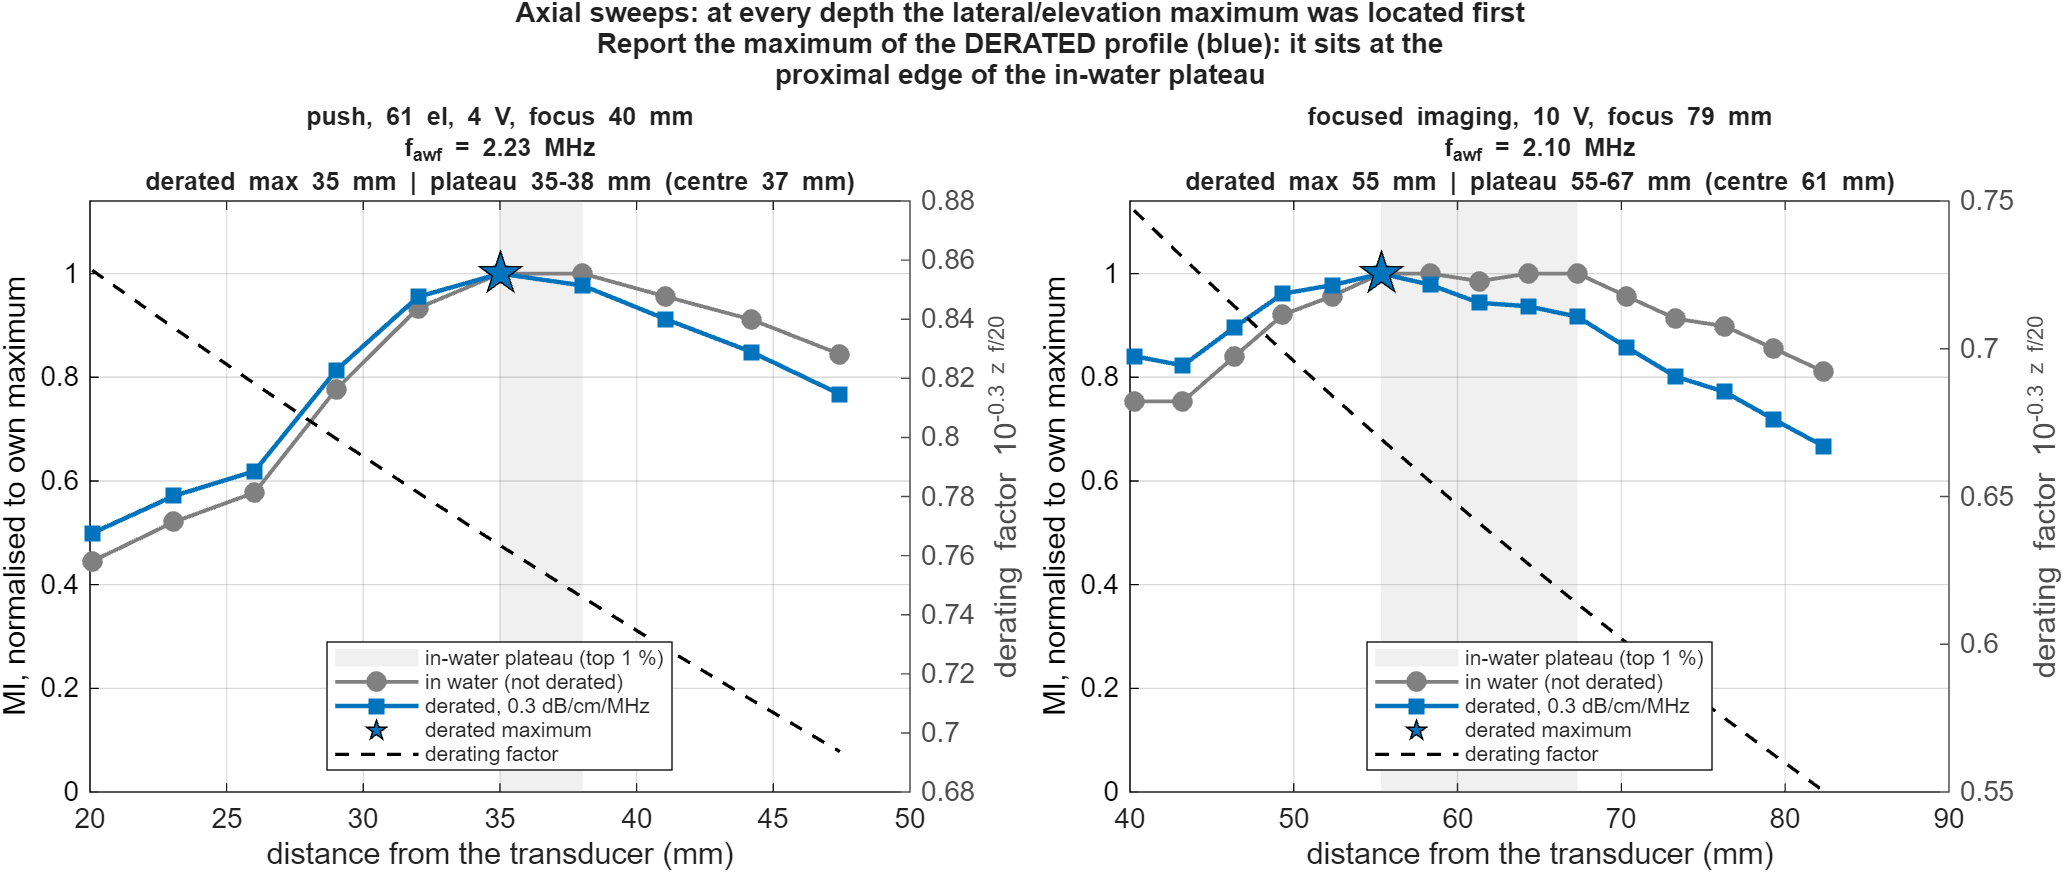
\includegraphics[width=\textwidth]{axial_deration.png}
\caption{Why the derated maximum has to be found rather than assumed. Two axial sweeps, each point
already the local lateral/elevation maximum. Grey: in water. Blue: after derating. Shaded: the depths
within $1\,\%$ of the in-water maximum. Dashed (right axis): the derating factor, which falls
monotonically with depth and tilts the profile proximal. \emph{Left:} a shallow
\SI{40}{\milli\metre}-focus push, where the shift is modest. \emph{Right:} a
\SI{79}{\milli\metre}-focus imaging beam, whose in-water field is a \SI{12}{\milli\metre}-wide
plateau and whose \emph{derated} maximum sits at the shallow edge of it,
\SI{24}{\milli\metre} proximal of the nominal focus. The plateau is \good{real, not a sampling
artefact}: at $F_\#=3.9$ and \SI{2.1}{\mega\hertz} the $-6$\,dB depth of focus is
$7.1F_\#^2\lambda\approx\SI{77}{\milli\metre}$, so the field genuinely varies by less than a per cent
over the \SI{12}{\milli\metre} shaded span. What the 8-bit digitizer contributes is only that
neighbouring stations then return \emph{bit-identical} codes (one code is \SI{0.7}{\percent} here),
which makes the in-water maximum unlocatable --- while the derated maximum stays sharp, for the
reason given in \S\ref{sec:stepsize}.}
\label{fig:axial}
\end{figure}

\subsection{Choosing the step sizes}\label{sec:stepsize}
Both the axial sweep and the transverse search at each station need a step small enough that the
recorded maximum really is the maximum.

\paragraph{Transverse (lateral and elevation).} Size the step as a \textbf{fraction of the beam
width}, never as an absolute distance. Modelling the focal-plane amplitude as a sinc of half-width
$\mathrm{FWHM}=1.21\,\lambda F_\#$, a square grid of step $\Delta$ can miss the peak by $\Delta/2$ in
both axes at once, costing $1-\mathrm{sinc}^2(\pi\Delta/2)$ in amplitude. A step of
$\mathrm{FWHM}/3$ costs up to \SI{13}{\percent} on MI and \SI{24}{\percent} on the intensities;
$\mathrm{FWHM}/10$ costs about \SI{1}{\percent}.

\begin{quote}
\textbf{Use $\Delta \le \mathrm{FWHM}/10$}, recomputed for every geometry, and sized \emph{per axis}
--- elevation is focused by a fixed lens, so its width differs from the lateral one and the narrower
of the two governs its own step.
\end{quote}

\noindent
Going finer than $\mathrm{FWHM}/10$ buys little: at \SI{1}{\percent} the error is already well below
the hydrophone calibration uncertainty, and the 8-bit digitizer's own quantisation floor is a few
tenths of a per cent. For our geometries this works out at \SIrange{0.1}{0.2}{\milli\metre} for the
S5-1 and about \SI{0.05}{\milli\metre} for the L11-5 at \SI{5}{\mega\hertz} --- tight enough that
stage resolution, not patience, becomes the limit, which is a further argument for the automated
raster of \S\ref{sec:ideal}.

\paragraph{Axial.} A few millimetres is enough. The derated profile falls monotonically across the
in-water plateau (a flat function times a monotonically decreasing one), so its maximum sits at the
sharp \emph{knee} where the rising flank meets the plateau, not somewhere unlocatable in the middle.
\SI{3}{\milli\metre} resolved that knee in both of our sweeps. Confirm it rather than assume it: fit
a parabola through the sampled maximum and its two neighbours --- near-symmetric neighbours mean the
step was fine enough, and the fitted vertex gives sub-step localisation for free, while strongly
asymmetric ones are the signal to refine.

\begin{mistake}
\mistaketitle{concluding from a flat local response that the step is fine enough}
Near the peak the response is genuinely flat --- a \SI{0.1}{\milli\metre} move changes the reading by
only \SI{0.5}{\percent}, which is easy to read as ``precise enough''. The trap is that the same move
costs \SI{7.6}{\percent} at \SI{0.6}{\milli\metre} off axis and \SI{14.5}{\percent} at
\SI{1.0}{\milli\metre}. \good{Large sensitivity to a small move is the diagnostic that you are on the
flank, not at the peak} --- keep refining until the response goes flat, and only then record.
\end{mistake}

\subsection{Step 4 --- sweep the transmit voltage at that point}
Park the hydrophone at the derated maximum and sweep the transmit voltage; this is the measurement
that becomes a permissible-voltage limit. Cover the linear region on chain A, and if the sequence
will be used above the clipping ceiling, repeat the high-voltage points on chain B, overlapping the
two chains over several voltages.

\subsection{Step 5 --- what to measure, and what to scale}\label{sec:scaling}
Re-measuring the whole field for every sequence variant is unnecessary:
\begin{itemize}
  \item \textbf{Changes the field shape $\rightarrow$ measure.} Beam type (focused / diverging /
    plane), aperture or element count, focal depth, transmit frequency. Each needs its own axial
    sweep, because each moves the maximum.
  \item \textbf{Scales predictably $\rightarrow$ measure once at the peak and scale.} Transmit
    voltage (MI $\propto V$, intensities $\propto V^2$, up to nonlinear saturation --- verify with a
    few points across the range); pulse length (scales $I_\mathrm{spta}$ only); PRF and duty cycle (a
    global multiplier on $I_\mathrm{spta}$).
\end{itemize}

\begin{mistake}
\mistaketitle{treating the long-time-average $I_\mathrm{spta}$ as the whole thermal story}
A burst duty cycle --- a second of pushing followed by tens of seconds of quiet --- makes the
regulatory $I_\mathrm{spta}$ small, and that is legitimate. But the transient temperature rise
\emph{within} each burst is a separate question that $I_\mathrm{spta}$ does not answer. Check the
thermal indices, and probe-face heating, separately.
\end{mistake}

% ======================================================================
\section{Checklist}\label{sec:checklist}
% ======================================================================
Run through this before starting, and again before reporting. The four groups below correspond to
the four places a measurement usually goes wrong: the electrical chain, the digitizer, the
positioning, and the reporting.

\newcommand{\ckhead}[1]{\multicolumn{2}{@{}l}{\textbf{#1}}\\[2pt]}
\newcommand{\ckitem}[1]{\hangindent=1.1em\hspace*{1.1em}#1}
{\small\setlength{\LTpre}{6pt}\setlength{\LTpost}{6pt}
\begin{longtable}{@{}>{\raggedright\arraybackslash}p{0.42\textwidth}>{\raggedright\arraybackslash}p{0.53\textwidth}@{}}
\toprule
\endhead
\ckhead{Electrical chain}
\ckitem{Scope impedance recorded, $2{:}1$ ratio verified} &
  A factor 2 on MI, 4 on the intensities, invisible in the waveform (\S\ref{sec:impedance}). \\
\ckitem{Waveforms inspected for flat tops} &
  Clipping is not obvious from the peak value alone (\S\ref{sec:clipping}). \\
\ckitem{No attenuator used to ``fix'' clipping} &
  The clipping stage is upstream of it; remove the pre-amplifier instead (\S\ref{sec:clipping}). \\
\ckitem{$C_\mathrm{load}$ re-determined after any cabling change} &
  It dominates the no-preamp reading and is not a datasheet value (\S\ref{sec:cloadcal}). \\
\addlinespace
\ckhead{Digitizer}
\ckitem{Real-time sampling, not RIS} &
  Equivalent-time sampling is invalid for a single-shot push (\S\ref{sec:scopesettings}). \\
\ckitem{Record length $>$ pulse length} &
  A truncated record silently under-reports PII and both intensities. \\
\ckitem{Vertical range re-checked after each voltage change} &
  8-bit digitizer; a loose range throws away resolution. \\
\ckitem{Full waveform saved, not just $V_\mathrm{pp}$} &
  Everything except $p_r$ needs the waveform (\S\ref{sec:savewaveform}). \\
\addlinespace
\ckhead{Positioning}
\ckitem{\texttt{Home} and \texttt{Pos} in every capture note} &
  Sets the derating depth; \SI{5}{\milli\metre} of origin error is already \SI{0.3}{\decibel}
  (\S\ref{sec:home}). \\
\ckitem{Transverse search at \emph{every} axial station, step $\le$ FWHM/10} &
  Otherwise a constant multiplicative under-read (\S\ref{sec:axial}, \S\ref{sec:stepsize}). \\
\ckitem{Axial sweep continued until the profile turns over} &
  The derated maximum is proximal of the in-water one (\S\ref{sec:axial}). \\
\ckitem{Bubbles checked on tip and lens; absorber in place for long bursts} &
  Both read low, and neither is visible in the number (\S\ref{sec:water}, \S\ref{sec:reflections}). \\
\addlinespace
\ckhead{Analysis and reporting}
\ckitem{$f_\mathrm{awf}$ from a low-drive capture, fundamental band only} &
  Harmonics inflate a wideband estimate as drive rises (\S\ref{sec:fawf}). \\
\ckitem{$p_r$ from the minimum, not $V_\mathrm{pp}/2$} &
  The waveform is nonlinearly asymmetric (\S\ref{sec:conversion}). \\
\ckitem{Local (per-point) PRF used for $I_\mathrm{spta}$} &
  For a scanned sequence that is the frame rate, not the line rate. \\
\ckitem{Application stated with every reported number} &
  $I_\mathrm{spta.3}$ ranges over $40\times$ between applications (\S\ref{sec:limits}). \\
\ckitem{Thermal indices checked separately for burst sequences} &
  $I_\mathrm{spta}$ does not capture the within-burst transient (\S\ref{sec:scaling}). \\
\bottomrule
\end{longtable}}


\section{Worked results}\label{sec:results}
% ======================================================================
This section reports our own measurements, as examples of what the protocol produces.

\subsection{Validation against Verasonics on the L11-5}\label{sec:l115}
Verasonics reports MI at a single location for a small number of its example scripts --- far from
all of them, but enough to validate the method against an independent reference. We used
\texttt{L11-5v High Image Quality} (\texttt{WideBeamHISC}), a harmonic pulse-inversion sequence
transmitting one cycle at \SI{4.46}{\mega\hertz}, received at
$f_\mathrm{awf}=\SI{5.0}{\mega\hertz}$, and measured at the reference depth of
\SI{11}{\milli\metre} over a \SIrange{2}{50}{\volt} transmit sweep, in all four combinations of pulse
polarity and scope impedance.

\begin{figure}[t]
\centering
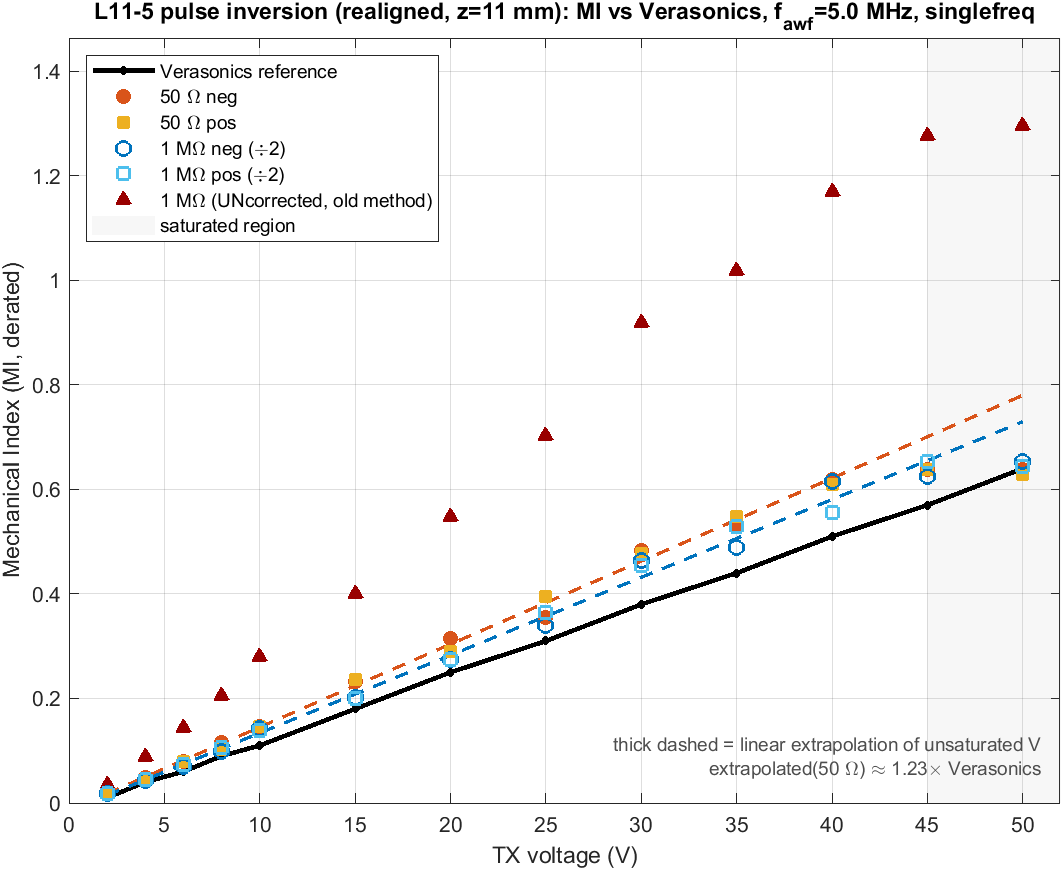
\includegraphics[width=0.84\textwidth]{L11_5_verasonics_comparison.png}
\caption{L11-5 pulse inversion at \SI{11}{\milli\metre}: measured MI versus transmit voltage against
the Verasonics reference (black). Circles and squares: the corrected analysis at \SI{50}{\ohm} and at
\SI{1}{\mega\ohm} with the $\div2$ load correction --- the four series coincide. Red triangles: the
same \SI{1}{\mega\ohm} data \emph{without} the load correction, running away to $2\times$. Shaded:
where the pre-amplifier saturates; dashed lines are linear extrapolations from the unsaturated
points.}
\label{fig:l115}
\end{figure}

Figure~\ref{fig:l115} validates four things at once:
\begin{itemize}
  \item \good{The impedance correction is right.} The \SI{50}{\ohm} and \SI{1}{\mega\ohm}$\div2$
    series coincide, while the uncorrected \SI{1}{\mega\ohm} points sit a clean factor $2$ high.
  \item \good{Normal and inverted pulses agree}, as they must for pulse inversion.
  \item \good{The shape is right}: MI is linear in transmit voltage with the same slope as the
    reference, over the whole unsaturated range.
  \item \good{The absolute value agrees to $1.23\times$}, roughly constant with voltage, after
    extrapolating the unsaturated ($\le\SI{30}{\volt}$) region.
\end{itemize}

\paragraph{On the residual $1.23\times$.} We could not remove it, having excluded: using the
programmed \SI{4.46}{\mega\hertz} rather than the measured \SI{5.0}{\mega\hertz} (which makes it
worse, $1.32\times$); spatial averaging by the \SI{400}{\micro\metre} tip (a few per cent, in the
wrong direction); broadband deconvolution (also the wrong direction); tank reflections (the echo at
$2\times\SI{11}{\milli\metre}/c\approx\SI{14.7}{\micro\second}$ falls outside the
\SI{5}{\micro\second} window); bubbles (they attenuate, and erratically, whereas this is a steady
over-read); and the derating depth. What remains is the absolute accuracy of the hydrophone
calibration ($\pm1$--\SI{2}{\decibel} is typical) and whatever model Verasonics uses;
$1.23\times$ is \SI{1.8}{\decibel}, within the combined uncertainty of the two. \caveat{Note the
direction:} we measure \emph{higher} than Verasonics, which is conservative for safety but means this
agreement cannot be used to argue our numbers are pessimistic.

\paragraph{Why the transverse search is in the protocol.} An earlier version of this dataset, taken
without re-aligning in elevation, gave MI a constant $0.36\times$ Verasonics --- a pure
multiplicative offset with the shape preserved, exactly the signature described in
\S\ref{sec:axial}. Re-aligning produced Figure~\ref{fig:l115}.

\subsection{S5-1 ARF push}\label{sec:s51}
The target measurement: the focused ARF push used for shear-wave elastography on the S5-1
(\SI{1.95}{\mega\hertz} programmed, $f_\mathrm{awf}=\SI{2.23}{\mega\hertz}$, focus
\SI{40}{\milli\metre}, 1900 cycles, apertures of 41 / 61 / 79 elements, burst duty of 24 pushes at
\SI{20}{\hertz} followed by $\ge\SI{30}{\second}$ off, i.e.\ \SI{0.77}{\hertz} effective). No
reference value exists for it anywhere.

\paragraph{Locating the maximum.} The axial sweep (Figure~\ref{fig:axial}, left) was run at
\SI{4}{\volt} in \SI{3}{\milli\metre} steps from \SIrange{20}{47}{\milli\metre}, with a transverse
search at every station. The derated maximum falls at $z\approx\SI{35}{\milli\metre}$, proximal of
the \SI{40}{\milli\metre} nominal focus, and is bracketed. Figure~\ref{fig:axialpre} repeats the
sweep on both chains: the two --- a factor $73$ apart in sensitivity --- agree on both the profile
and the location of the maximum, which is a useful end-to-end check.

\begin{figure}[h]
\centering
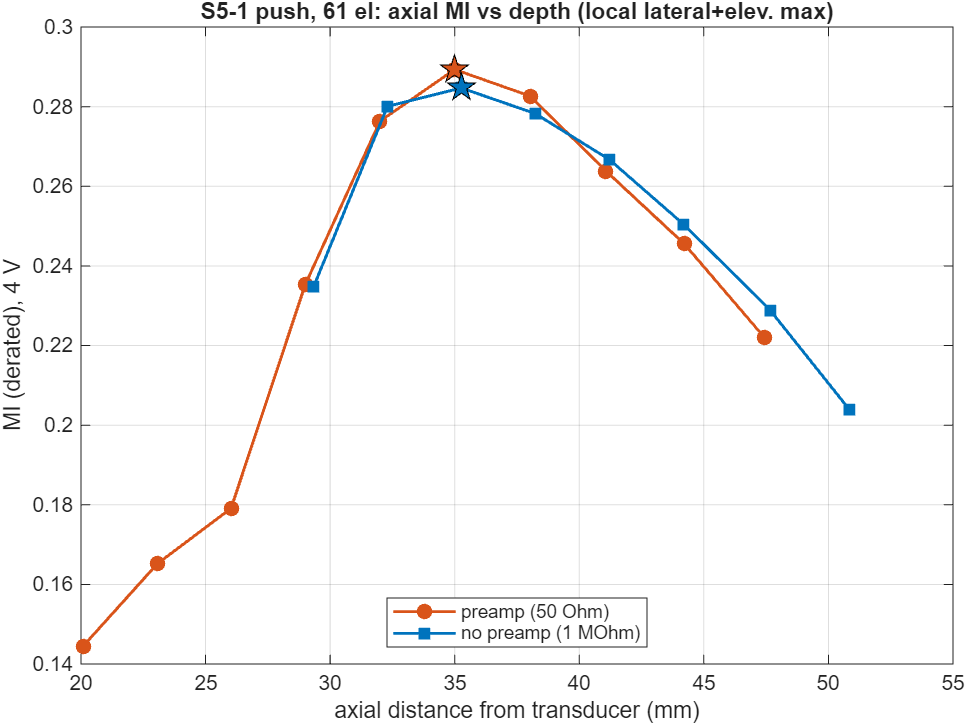
\includegraphics[width=0.66\textwidth]{push_axial_preamp.png}
\caption{The same axial sweep measured on both chains.}
\label{fig:axialpre}
\end{figure}

\paragraph{$C_\mathrm{load}$.} The procedure of \S\ref{sec:cloadcal} gave
$C_\mathrm{load}=\SI{123.3}{\pico\farad}$, constant over \SIrange{3}{12}{\volt} transmit. An
independent determination in the L11-5 session --- different probe, different frequency --- gave
\SI{121}{\pico\farad}, a $2\,\%$ agreement, which is the evidence behind the transferability claim in
\S\ref{sec:cloadcal}.

\paragraph{Voltage and aperture.} At the peak point the transmit voltage was swept from
\SIrange{2}{20}{\volt} on chain A and \SIrange{2}{50}{\volt} on chain B
(Figure~\ref{fig:vsweep}), and the sweep repeated at 41, 61 and 79 elements
(Figures~\ref{fig:elements} and \ref{fig:intensities}). Chain A is usable to
$\approx\SI{10}{\volt}$; chain B runs to the full \SI{50}{\volt} and agrees with chain A where they
overlap.

\begin{figure}[h]
\centering
\begin{subfigure}[b]{0.48\textwidth}
  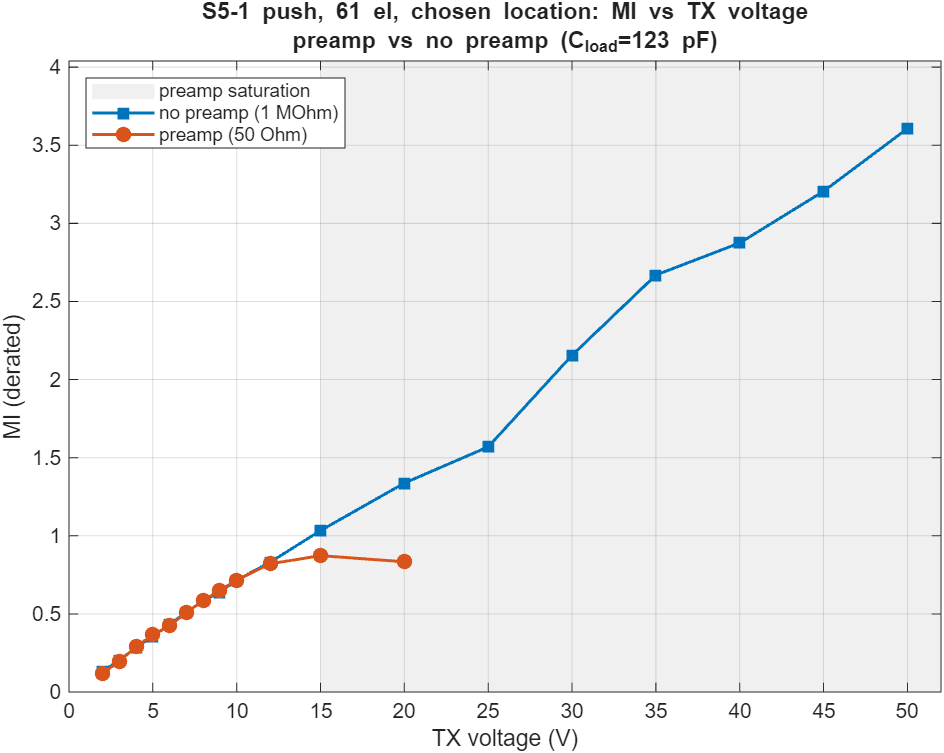
\includegraphics[width=\textwidth]{push_voltage_preamp.png}
  \caption{MI versus transmit voltage on both chains. The shaded region is where chain A saturates.}
  \label{fig:vsweep}
\end{subfigure}\hfill
\begin{subfigure}[b]{0.48\textwidth}
  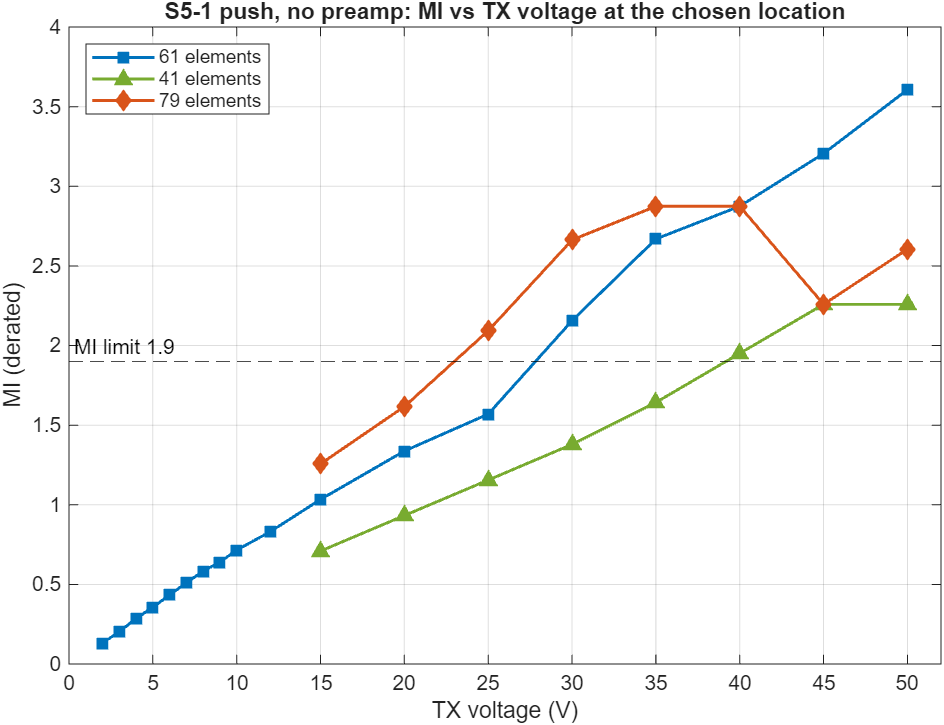
\includegraphics[width=\textwidth]{push_voltage_elements.png}
  \caption{MI versus transmit voltage for the three apertures, chain B. MI crosses $1.9$ at
  \SI{39}{\volt} (41 el), \SI{28}{\volt} (61 el) and \SI{23}{\volt} (79 el).}
  \label{fig:elements}
\end{subfigure}
\caption{S5-1 push voltage sweeps at the derated field maximum. \caveat{The non-monotonic points
above $\approx\SI{40}{\volt}$} are single captures in a strongly shocked, supply-sagging regime and
are not reliable; they lie far above every limit crossing.}
\end{figure}

\begin{figure}[t]
\centering
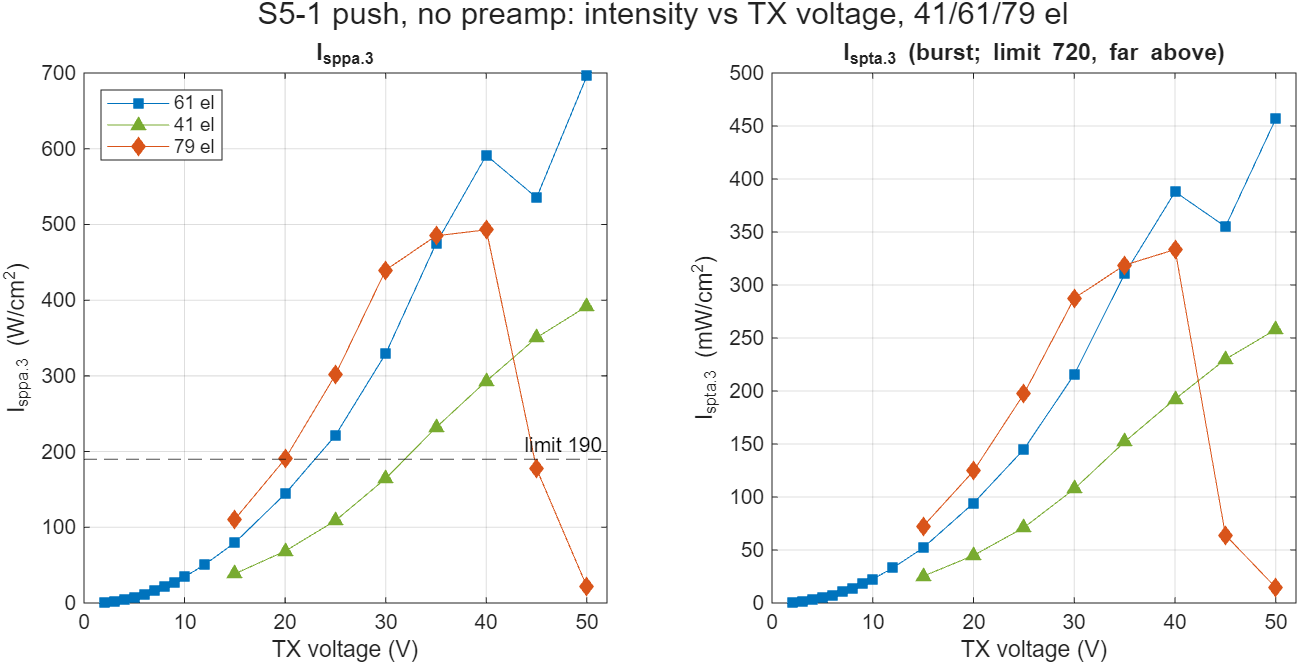
\includegraphics[width=\textwidth]{push_intensity_elements.png}
\caption{The two intensities for the same three apertures. \emph{Left:} $I_\mathrm{sppa.3}$ crosses
\SI{190}{\watt\per\square\centi\metre} at \SIrange{20}{32}{\volt}. \emph{Right:} $I_\mathrm{spta.3}$
at those voltages is only \SIrange{100}{190}{\milli\watt\per\square\centi\metre}, entirely because of
the burst duty cycle. Above $\approx\SI{40}{\volt}$ the $10$--$90\,\%$ window that defines the pulse
duration becomes unstable on a shocked waveform --- at \SI{45}{\volt} it returns
\SI{470}{\micro\second} for an \SI{850}{\micro\second} burst --- which is what produces the apparent
collapse of the 79-element curve.}
\label{fig:intensities}
\end{figure}

\begin{table}[t]
\centering
\caption{Maximum permissible transmit voltage for the S5-1 push at the derated field maximum
($z\approx\SI{36}{\milli\metre}$, 1900 cycles, burst duty \SI{0.77}{\hertz} effective), from the
chain-B measurements, requiring \emph{both} MI $\le1.9$ and
$I_\mathrm{sppa.3}\le\SI{190}{\watt\per\square\centi\metre}$.}
\label{tab:maxv}
\begin{tabular}{lccccl}
\toprule
Aperture & $V$ at MI $=1.9$ & $V$ at $I_\mathrm{sppa.3}=190$ & $V$ at $I_\mathrm{spta.3}=720$
  & \textbf{max $V$} & Binding limit \\
\midrule
41 elements & \SI{39.3}{\volt} & \SI{32.0}{\volt} & $>\SI{50}{\volt}$ & \textbf{\SI{32}{\volt}} & $I_\mathrm{sppa.3}$ \\
61 elements & \SI{27.9}{\volt} & \SI{23.1}{\volt} & $>\SI{50}{\volt}$ & \textbf{\SI{23}{\volt}} & $I_\mathrm{sppa.3}$ \\
79 elements & \SI{23.1}{\volt} & \SI{20.1}{\volt} & $>\SI{50}{\volt}$ & \textbf{\SI{20}{\volt}} & $I_\mathrm{sppa.3}$ \\
\bottomrule
\end{tabular}
\end{table}

\paragraph{Outcome.} Table~\ref{tab:maxv} gives the crossings. Four observations that generalise:
\begin{itemize}
  \item \good{$I_\mathrm{sppa.3}$ binds before MI} for these long focused pushes: at the permissible
    voltage MI is only $\approx1.5$--$1.6$. Checking MI alone --- the index everyone quotes ---
    overshoots by \SIrange{15}{25}{\percent} in voltage. (Under a strict reading of the \textbf{or}
    in Table~\ref{tab:fdalimits} the MI crossing would be the operative one; we require both.)
  \item \good{The burst duty is what buys the $I_\mathrm{spta}$ headroom.} At the permissible
    voltages $I_\mathrm{spta.3}$ sits near \SI{100}{\milli\watt\per\square\centi\metre} --- under
    both the \SI{720}{} and the cardiac \SI{430}{\milli\watt\per\square\centi\metre} limit. Change
    the duty cycle and this is the first number to recompute.
  \item \good{Extrapolation from an unsaturated region works.} A separate analysis fitting only
    the low-voltage chain-A sweep and extrapolating ($\mathrm{MI}\propto V$,
    $I_\mathrm{sppa}\propto V^2$) predicted \SI{20.0}{\volt} for 79 elements and \SI{24.3}{\volt} for
    61 --- within \SI{6}{\percent} of the directly measured values. It worked here because the limits
    are crossed at \SIrange{20}{32}{\volt}, below where saturation bites.
  \item \caveat{But the two chains are not independent, and this is not an absolute check.}
    $C_\mathrm{load}$ was solved from the chain-A/chain-B voltage ratio (\S\ref{sec:cloadcal}), so
    chain~B's pressure scale is derived from chain~A's calibration. An error in the preamp-chain
    sensitivity --- above all in the hydrophone sensitivity $M_c$, the one term carrying
    \SIrange{1}{2}{\decibel} of uncertainty --- propagates into $C_\mathrm{load}$ and then into
    every no-preamp number, by the same factor, and cannot show up in this comparison. What the
    agreement does establish is that the extrapolation is sound and that neither chain is distorted
    by saturation at the crossing voltages. \good{Testing the absolute scale needs a second,
    independently calibrated hydrophone} --- see \S\ref{sec:l115}, where the residual
    $1.23\times$ against Verasonics is exactly the kind of error this comparison is blind to.
  \item \caveat{The table is deliberately pessimistic.} It is built from the peak-optimised single
    captures at each voltage, which read higher than repeated captures at the same nominal position
    (\SI{102}{\milli\volt} versus \SI{66}{\milli\volt} at \SI{40}{\volt}, 79 elements). That is the
    correct conservative choice for a limit, but it should not be quoted as the typical output.
\end{itemize}

\section{Code and data}\label{sec:files}
% ======================================================================
Everything this document refers to --- the code, the calibration, and the raw \texttt{.hws} captures
behind every figure and every number in \S\ref{sec:results} --- is in the repository this report
lives in. There is no external dependency and no absolute path: clone it, run \texttt{misetup}, and
every script finds its own data.

\begin{center}
\begin{tabular}{ll}
\toprule
\texttt{docs/report/}          & this document and its figures \\
\texttt{code/readHWS.m}        & read an \texttt{.hws} capture (waveform $+$ config $+$ note) \\
\texttt{code/SafetyIndices.m}  & waveform $\rightarrow$ MI, $I_\mathrm{sppa.3}$, $I_\mathrm{spta.3}$ \\
\texttt{code/SystemSensitivity.m} & calibration $\rightarrow$ \si{\volt\per\mega\pascal}, either chain \\
\texttt{code/analysis/}        & the full analyses, including \texttt{MakeReportFigures} \\
\texttt{calibration/}          & the two Onda certificates (source of truth) and the digested tables \\
\texttt{data/}                 & the captures used here, with the acquisition note inside each file \\
\texttt{demo/RunDemo.m}        & an end-to-end worked example that checks itself \\
\bottomrule
\end{tabular}
\end{center}

\noindent To reproduce the figures of this report:

\begin{quote}\ttfamily
misetup \\
MakeReportFigures
\end{quote}

\noindent
\texttt{RunDemo} is the fastest way to see the whole chain work on real data; it ends by comparing
every quantity it computed against stored reference values, so a broken installation announces
itself rather than producing plausible wrong numbers.


\appendix
% ----------------------------------------------------------------------
%  Appendix: operating the OWIS motion stage.
%  Adapted from L. van Knippenberg, "OWIS motion stage -- How to setup and
%  use" (19 March 2024). Figures extracted from that document.
%  NOTE: the installation password in the original is deliberately NOT
%  reproduced here -- see the remark in the setup subsection.
% ----------------------------------------------------------------------
\section{Operating the OWIS motion stage}\label{app:owis}

The hydrophone is carried by an OWIS three-axis motion stage (Figure~\ref{fig:owisstage}),
driven from OWISoft on the Vantage~256 PC. Every coordinate in this report ---
\texttt{Home}, \texttt{Pos}, the axial step, the transverse search --- is a stage coordinate, so
this appendix records how to drive it. It is a condensed version of the standalone note
\emph{OWIS motion stage --- how to setup and use} (19~March~2024); the OWISoft and PS-10 manuals
are the reference for anything beyond this, and are on the group NAS alongside the installer at
\texttt{Ultrasound-BMd\textbackslash Software\textbackslash OWIsoft}.

\begin{figure}[h]
\centering
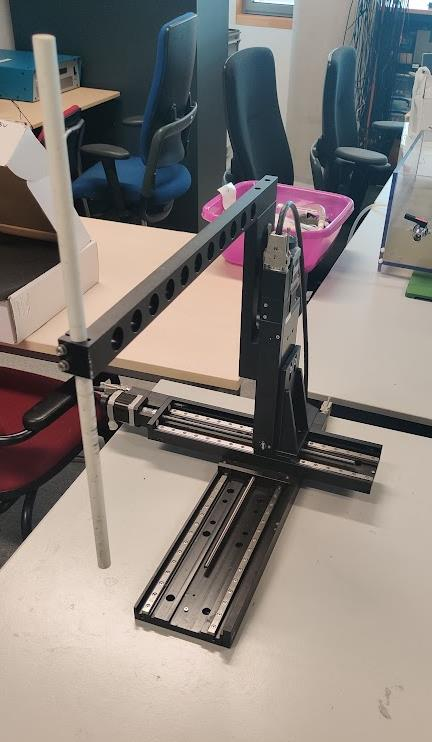
\includegraphics[height=6.2cm]{owis_stage.jpeg}
\caption{The OWIS three-axis motion stage, with the hydrophone holder mounted vertically.}
\label{fig:owisstage}
\end{figure}

\subsection{Starting up}
\begin{enumerate}[leftmargin=*]
  \item On the Vantage~256 PC, start \textbf{OWISoft} (Desktop $\rightarrow$ \texttt{OWIsoft}
    folder).
  \item Open all three control units: \textbf{File $\rightarrow$ Control unit $\rightarrow$ Open},
    and take \texttt{X}, \texttt{Y} and \texttt{Z} from the default folder.
  \item \textbf{Tick \emph{active} for all three} (Figure~\ref{fig:owisfree}, left). An axis that is
    not activated silently ignores every move command.
\end{enumerate}

\subsection{Free positioning --- moving by hand}
The \textbf{Free positioning} tab (Figure~\ref{fig:owisfree}) is what the whole measurement of
\S\ref{sec:protocol} is driven from. Enter a displacement per axis and press \textbf{Move relative},
or an absolute coordinate and \textbf{Move absolute}; several axes may move at once. In the example
shown the stage would advance \SI{5}{\milli\metre} in $x$.

\good{Use \emph{Set home position} once the hydrophone tip is at the centre of the transducer face},
and the stage will return there with \emph{Move to home position}. That point is the
\texttt{Home} of \S\ref{sec:home}, and the derating depth of every capture is measured from it, so
setting it deliberately at the start of a session is what makes the rest of the geometry meaningful.

\begin{figure}[h]
\centering
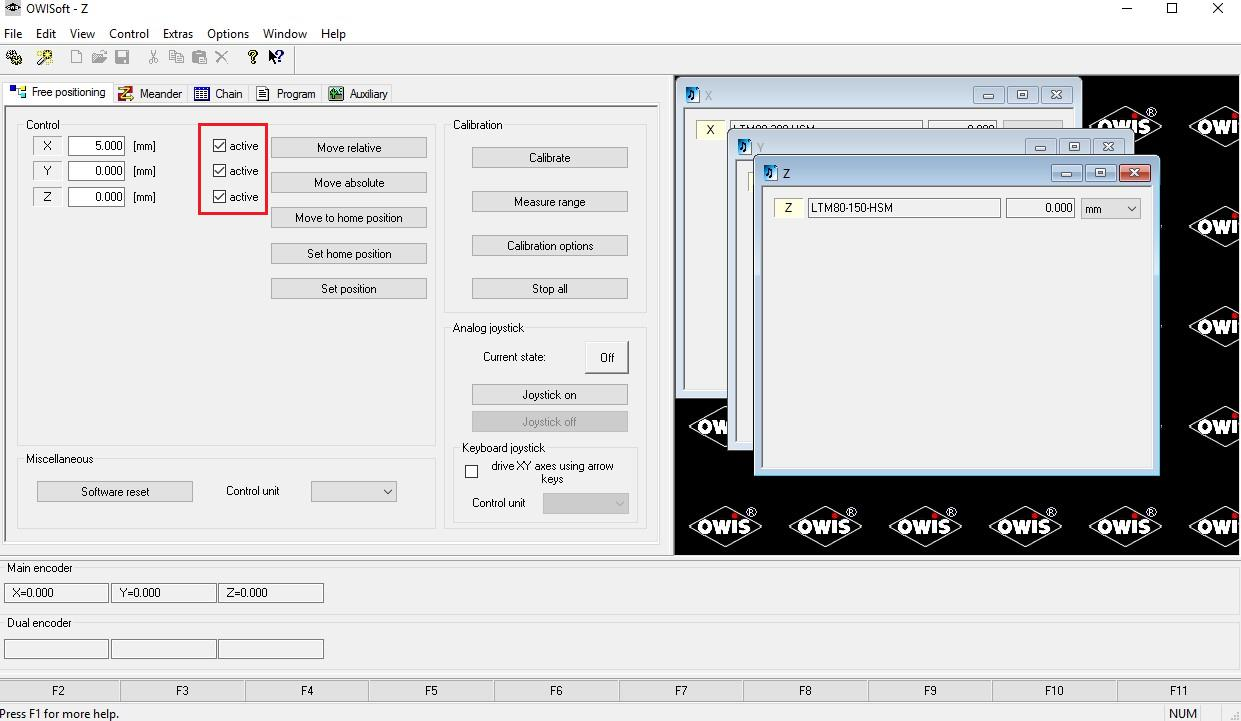
\includegraphics[width=\textwidth]{owis_freepos.jpeg}
\caption{Free positioning. Left: the three axes, each with its \emph{active} checkbox --- all three
must be ticked. \emph{Set home position} defines the \texttt{Home} used throughout this report.}
\label{fig:owisfree}
\end{figure}

\subsection{Meander --- scanning a grid automatically}
The \textbf{Meander} tab (Figure~\ref{fig:owismeander}) cycles through a rectangular grid defined by
a step count and a step length per axis, moving in $x$ first, then $y$, then $z$. Between points it
waits for a fixed delay, a mouse click, or the completion of a custom function.

This is the mechanism the automated 3-D raster of \S\ref{sec:ideal} would be built on. What is
missing is not the motion --- it is the synchronisation: the meander must trigger the digitizer and
wait for a capture to be written before stepping on. The \emph{wait for function} option is the hook
for that.

\begin{figure}[h]
\centering
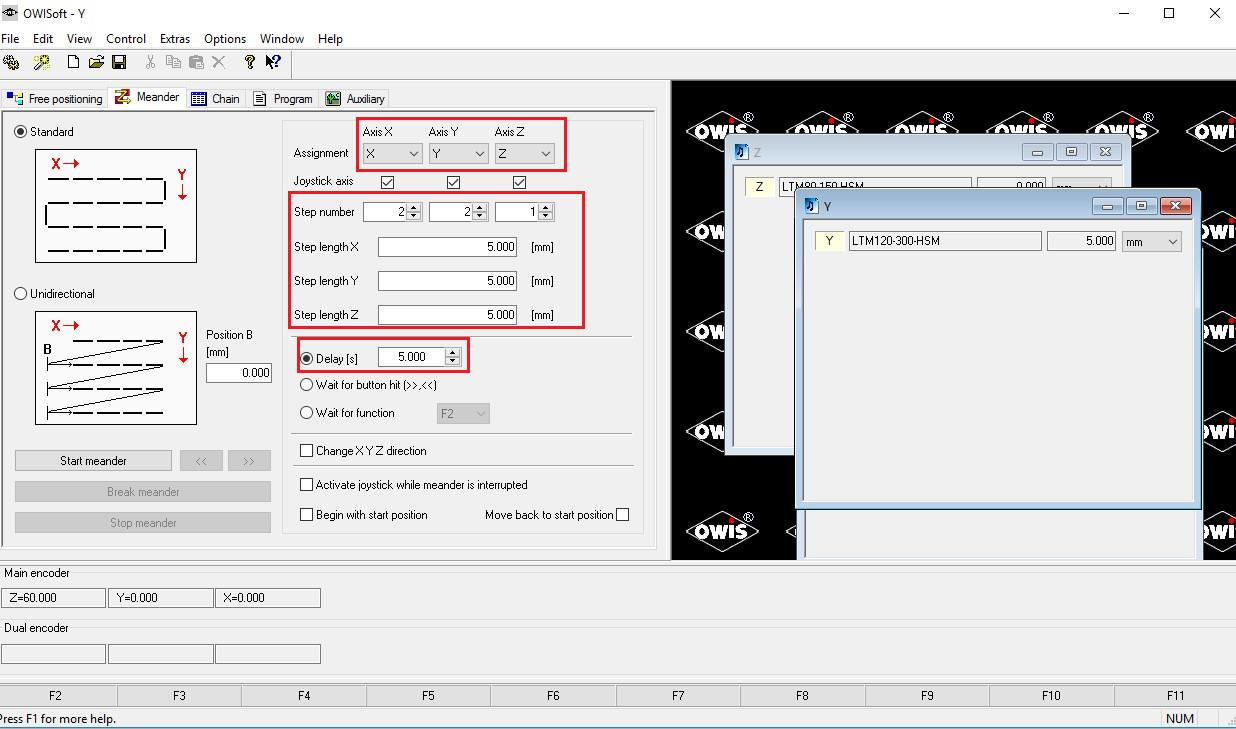
\includegraphics[width=\textwidth]{owis_meander.jpeg}
\caption{Meander. The grid comes from the step count and step length per axis; the dwell between
points is a fixed delay, a button press, or a custom function --- the last being the hook a
synchronised raster would use.}
\label{fig:owismeander}
\end{figure}

\subsection{First-time setup}
\emph{Reference only --- this was done on the Vantage system on 19~March~2024 and does not need
repeating unless the PC or the controllers are replaced.}

\begin{enumerate}[leftmargin=*]
  \item \textbf{Install OWISoft}. The installer and the OWIS manuals are on the group NAS at
    \texttt{Ultrasound-BMd\textbackslash Software\textbackslash OWIsoft}; they are licensed
    software and are deliberately not in this repository. Setup asks for a user name, a company
    and an installation password --- \caveat{the password is not reproduced here}, it is with
    the installer on the NAS.
  \item \textbf{Configure three control units}, one per axis: \textbf{File $\rightarrow$ Control
    unit $\rightarrow$ New} (Figure~\ref{fig:owisconnect}), then
    \begin{itemize}
      \item select the COM port --- if unsure which is which, unplug the units one at a time and
        see which port disappears;
      \item set \textbf{Control unit type} to \texttt{PS10};
      \item tick \emph{Initialize axes automatically} and \emph{Connect automatically at startup};
      \item press \textbf{Connect}.
    \end{itemize}
  \item An axis-configuration wizard opens (Figure~\ref{fig:owisaxis}):
    \begin{itemize}
      \item under \textbf{Step 1}, \emph{Show dialog box}, and name the axis (axis 1 $\rightarrow$
        \texttt{X});
      \item \emph{Identify} finds the positioning-unit type number;
      \item \emph{Auto-configuration}, then close;
      \item under \textbf{Step 5}, \emph{Initialize}, then close.
    \end{itemize}
    Repeat for \texttt{Y} and \texttt{Z}.
  \item \textbf{Save}: File $\rightarrow$ Control unit $\rightarrow$ Save.
\end{enumerate}

\begin{figure}[h]
\centering
\begin{subfigure}[t]{0.40\textwidth}
  \centering
  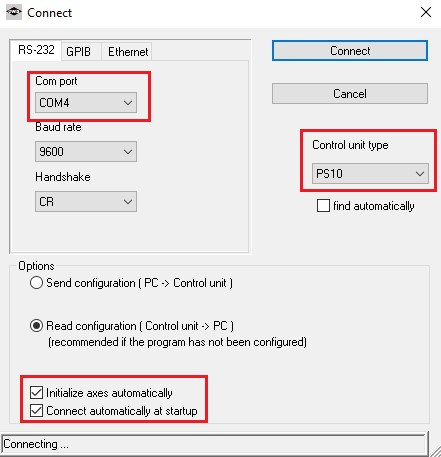
\includegraphics[width=\textwidth]{owis_connect.png}
  \caption{Connecting a control unit.}
  \label{fig:owisconnect}
\end{subfigure}\hfill
\begin{subfigure}[t]{0.56\textwidth}
  \centering
  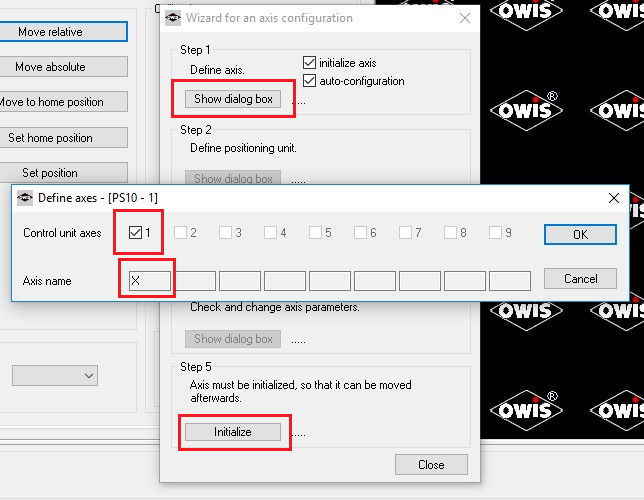
\includegraphics[width=\textwidth]{owis_axis.png}
  \caption{Configuring an axis.}
  \label{fig:owisaxis}
\end{subfigure}
\caption{First-time setup of one axis. Repeat for all three.}
\label{fig:owissetup}
\end{figure}


\end{document}
